%Fred, Simon, Sou-Cheng, Yuhan, NSF Grant Dec 2022
% GitHub: https://github.com/fjhickernell/NSF_CompMath2018Nov
% Overleaf: https://www.overleaf.com/9576964687whkhbmrrvhsd
\documentclass[11pt]{NSFamsart}
%\usepackage[top=1in,bottom=1in,left=1in,right=1in]{geometry}
\usepackage{latexsym,amsfonts,amsmath,amssymb,amsthm,epsfig,extdash,multirow}
\usepackage{stackrel,tabularx,mathtools,longtable,xspace}
\usepackage[shortlabels]{enumitem}
\usepackage[dvipsnames]{xcolor}
\usepackage[numbers,sort&compress]{natbib}
\usepackage{hyperref}
\usepackage{accents, booktabs}
\usepackage{algorithm, algorithmicx}
\usepackage{anyfontsize}
\usepackage[capitalise]{cleveref}
\usepackage{wrapfig}
\usepackage[font=small,labelfont=bf]{caption}
\usepackage[normalem]{ulem}

\voffset 0.23in
\hoffset 0in
\textheight 8.9in
\textwidth6.45in
\setlength{\oddsidemargin}{0in}
\setlength{\evensidemargin}{0in}
\headsep-0.6in
\thispagestyle{empty} \pagestyle{empty} %to eliminate page numbers for upload
\thispagestyle{plain} \pagestyle{plain} %to add back page numbers
\renewcommand{\baselinestretch}{0.98} %to squeeze the lines a bit

\crefname{section}{Sect.}{Sects.}
\crefname{figure}{Fig.}{Figs.}


\usepackage{minted}
\newminted{python}{frame=lines,framerule=1.5pt,breaklines=true}
\newmintinline[pyinline]{python}{}


\usepackage{algpseudocode}
\algnewcommand\algorithmicparam{\textbf{Parameters:}}
\algnewcommand\PARAM{\item[\algorithmicparam]}
\algnewcommand\algorithmicinput{\textbf{Input:}}
\algnewcommand\INPUT{\item[\algorithmicinput]}
%\algnewcommand\STATE{\item}
\algnewcommand\RETURN{\State \textbf{Return }}

%\usepackage{showlabels}
\newcommand{\Upara}[1]{\noindent\underline{#1}:\xspace}
\newcommand{\cmtS}[1]{{\color{blue}{(Simon: #1)}}}

\newcommand{\myshade}{60}
\colorlet{mylinkcolor}{violet}
\colorlet{mycitecolor}{violet}
%\colorlet{mycitecolor}{OliveGreen}
\colorlet{myurlcolor}{YellowOrange}

\hypersetup{
	linkcolor  = mylinkcolor!\myshade!black,
	citecolor  = mycitecolor!\myshade!black,
	urlcolor   = myurlcolor!\myshade!black,
	colorlinks = true,
}


% This package prints the labels in the margin
%\usepackage[notref,notcite]{showkeys}


%%list of acronyms with links
\newcommand{\FH}{\hyperlink{FHlink}{FH}\xspace}
\newcommand{\SM}{\hyperlink{SMlink}{SM}\xspace}
\newcommand{\SCTC}{\hyperlink{SCTClink}{SCTC}\xspace}
\newcommand{\AO}{\hyperlink{AOlink}{AO}\xspace}
\newcommand{\MM}{\hyperlink{MMlink}{MM}\xspace}
\newcommand{\CH}{\hyperlink{CHlink}{CH}\xspace}
\newcommand{\TS}{\hyperlink{TSlink}{TS}\xspace}
\newcommand{\IJi}{\hyperlink{IJlink}{IJ}\xspace}
\newcommand{\TT}{\hyperlink{TTlink}{TT}\xspace}
\newcommand{\RZ}{\hyperlink{RZlink}{RZ}\xspace}
\newcommand{\GEF}{\hyperlink{GEFlink}{GEF}\xspace}
\newcommand{\YD}{\hyperlink{YDlink}{YD}\xspace}
\newcommand{\JR}{\hyperlink{JRlink}{JR}\xspace}
\newcommand{\LlAJR}{\hyperlink{LlAJRlink}{LlAJR}\xspace}
\newcommand{\LD}{\hyperlink{LDlink}{LD}\xspace}
\newcommand{\LJ}{\hyperlink{LJlink}{LJ}\xspace}
\newcommand{\XT}{\hyperlink{XTlink}{XT}\xspace}
\newcommand{\KZ}{\hyperlink{KZlink}{KZ}\xspace}
\newcommand{\DL}{\hyperlink{DLlink}{DL}\xspace}
\newcommand{\XZ}{\hyperlink{XZlink}{KZ}\xspace}
\newcommand{\JL}{\hyperlink{JLlink}{JL}\xspace}
\newcommand{\YZ}{\hyperlink{YZlink}{YZ}\xspace}
\newcommand{\AS}{\hyperlink{ASlink}{AS}\xspace}
\newcommand{\CLT}{\hyperlink{CLTlink}{CLT}\xspace}
\newcommand{\PN}{\hyperlink{PNlink}{PN}\xspace}
\newcommand{\PR}{\hyperlink{PRlink}{PR}\xspace}
\newcommand{\DN}{\hyperlink{DNlink}{DN}\xspace}
\newcommand{\BO}{\hyperlink{BOlink}{BO}\xspace}
\newcommand{\QMC}{\hyperlink{QMClink}{QMC}\xspace}

\newcommand{\SEC}{Sect.\xspace}


\newcommand{\QMCSoft}{QMCSoft\xspace}
\newcommand{\QMCPy}{QMCPy\xspace}
\newcommand{\GAIL}{GAIL\xspace}
%\newcommand{\QMC}{QMC\xspace}
\newcommand{\IIDMC}{IID MC\xspace}
\newcommand{\SAMSIQMC}{SAMSI-QMC\xspace}
\newcommand{\SciPy}{SciPy\xspace}
\newcommand{\TensorFlow}{TensorFlow\xspace}
\newcommand{\GSL}{GSL\xspace}
\newcommand{\NAG}{NAG\xspace}
\newcommand{\MATLAB}{MATLAB\xspace}
\newcommand{\PyTorch}{PyTorch\xspace}
\newcommand{\Chebfun}{Chebfun\xspace}
\newcommand{\Rlang}{R\xspace}
\newcommand{\Julia}{Julia\xspace}


%\textheight9.1in

\newtheorem{theorem}{Theorem}


\providecommand{\FJHickernell}{Hickernell}
\newcommand{\hf}{\widehat{f}}
\newcommand{\hg}{\widehat{g}}
\newcommand{\hI}{\hat{I}}
\newcommand{\hatf}{\hat{f}}
\newcommand{\hatg}{\hat{g}}
\newcommand{\tf}{\widetilde{f}}
\newcommand{\tbf}{\tilde{\bff}}
%\DeclareMathOperator{\Pr}{\mathbb{P}}

% Math operators
\DeclareMathOperator{\std}{std}
\DeclareMathOperator{\cost}{COST}
\DeclareMathOperator{\comp}{COMP}
\DeclareMathOperator{\loss}{loss}
\DeclareMathOperator{\lof}{lof}
\DeclareMathOperator{\reg}{reg}
\DeclareMathOperator{\CV}{CV}
\DeclareMathOperator{\size}{wd}
\DeclareMathOperator{\GP}{\mathcal{G} \! \mathcal{P}}
\DeclareMathOperator{\erf}{erf}
\DeclareMathOperator*{\argmax}{arg\,max}
\DeclareMathOperator*{\argmin}{arg\,min}
\DeclareMathOperator{\QOI}{QOI} %Quantity of Interest
\DeclareMathOperator{\POI}{POI} %Parameter of Interest
\DeclareMathOperator{\Ans}{ANS}
\DeclareMathOperator{\Var}{Var}
\DeclareMathOperator{\APP}{\widehat{\QOI}}
\DeclareMathOperator{\SURR}{SM} %surrogate model
\DeclareMathOperator{\STREND}{ST} %surrogate trend
\DeclareMathOperator{\SVAR}{SV} %surrogate variation
\DeclareMathOperator{\SVARERR}{SVU} %surrogate variation uncertainty
\newcommand{\MLS}{\textrm{MLS}\xspace} %distance weighted least squares, also known as moving least squares
%\DeclareMathOperator{\ALG}{ALG}
\DeclareMathOperator{\ERR}{ERR}
\DeclareMathOperator{\VAL}{ACQ}
\DeclareMathOperator{\OPER}{OPER}
\DeclareMathOperator{\INT}{INT}
\DeclareMathOperator{\MIN}{MIN}
\DeclareMathOperator{\ID}{ID}
\DeclareMathOperator{\APPMIN}{\widehat{\MIN}}
\DeclareMathOperator{\APPID}{\widehat{\ID}}
\DeclareMathOperator{\MINVAL}{MINACQ}
\DeclareMathOperator{\IDVAL}{IDACQ}
\DeclareMathOperator{\SURRERR}{SU}
\DeclareMathOperator{\MINERR}{MERR}
\DeclareMathOperator{\IDERR}{IDERR}
\DeclareMathOperator{\Prob}{\mathbb{P}}
\DeclareMathOperator{\diag}{diag}
\DeclareMathOperator{\dist}{dist}
\DeclareMathOperator{\filldis}{fill}
\DeclareMathOperator{\sep}{sep}
\DeclareMathOperator{\avg}{avg}
\DeclareMathOperator{\vol}{vol}
\DeclareMathOperator{\cov}{cov}
\newcommand{\TREND}{\textup{T}}
\newcommand{\VAR}{\textup{V}}
\newcommand{\LS}{\textup{LS}}
\newcommand{\unif}{\textup{unif}}
\newcommand{\fidparam}{\bldeta}







\newcommand{\reals}{{\mathbb{R}}}
\newcommand{\naturals}{{\mathbb{N}}}
\newcommand{\natzero}{{\mathbb{N}_0}}
\newcommand{\integers}{{\mathbb{Z}}}
\def\expect{{\mathbb{E}}}
\def\il{\left \langle}
\def\ir{\right \rangle}
\def\e{\varepsilon}
\def\g{\gamma}
\def\l{\lambda}
\def\b{\beta}
\def\a{\alpha}
\def\lall{\Lambda^{{\rm all}}}
\def\lstd{\Lambda^{{\rm std}}}

\newcommand{\vf}{\boldsymbol{f}}
\newcommand{\hV}{\widehat{V}}
\newcommand{\tV}{\widetilde{V}}
\newcommand{\fraku}{\mathfrak{u}}
\newcommand{\hcut}{\mathfrak{h}}
\newcommand{\tOmega}{\widetilde{\Omega}}
\newcommand{\tvarrho}{\widetilde{\varrho}}

\newcommand{\bbE}{\mathbb{E}}
\newcommand{\tQ}{\widetilde{Q}}
\newcommand{\mA}{\mathsf{A}}
\newcommand{\mB}{\mathsf{B}}
\newcommand{\mC}{\mathsf{C}}
\newcommand{\mD}{\mathsf{D}}
\newcommand{\mG}{\mathsf{G}}
\newcommand{\mH}{\mathsf{H}}
\newcommand{\mI}{\mathsf{I}}
\newcommand{\bbK}{\mathbb{K}}
\newcommand{\mK}{\mathsf{K}}
\newcommand{\tmK}{\widetilde{\mathsf{K}}}
\newcommand{\mL}{\mathsf{L}}
\newcommand{\mM}{\mathsf{M}}
\newcommand{\mP}{\mathsf{P}}
\newcommand{\mQ}{\mathsf{Q}}
\newcommand{\mR}{\mathsf{R}}
\newcommand{\mX}{\mathsf{X}}
\newcommand{\mPhi}{\mathsf{\Phi}}
\newcommand{\mPsi}{\mathsf{\Psi}}
\newcommand{\mLambda}{\mathsf{\Lambda}}
\newcommand{\mSigma}{\mathsf{\Sigma}}
\newcommand{\cube}{[0,1]^d}
\newcommand{\design}{\{\bx_i\}_{i=1}^n}




\newcommand{\bone}{\boldsymbol{1}}
\newcommand{\bzero}{\boldsymbol{0}}
\newcommand{\binf}{\boldsymbol{\infty}}
\newcommand{\ba}{{\boldsymbol{a}}}
\newcommand{\bb}{{\boldsymbol{b}}}
\newcommand{\bc}{{\boldsymbol{c}}}
\newcommand{\bd}{{\boldsymbol{d}}}
\newcommand{\be}{{\boldsymbol{e}}}
\newcommand{\bff}{{\boldsymbol{f}}}
\newcommand{\bhh}{{\boldsymbol{h}}}
\newcommand{\beps}{{\boldsymbol{\varepsilon}}}
\newcommand{\tbeps}{\tilde{\beps}}
\newcommand{\bt}{{\boldsymbol{t}}}
\newcommand{\bT}{{\boldsymbol{T}}}
\newcommand{\bx}{{\boldsymbol{x}}}
\newcommand{\bX}{{\boldsymbol{X}}}
\newcommand{\bh}{{\boldsymbol{h}}}
\newcommand{\bj}{{\boldsymbol{j}}}
\newcommand{\bk}{{\boldsymbol{k}}}
\newcommand{\bg}{{\boldsymbol{g}}}
\newcommand{\bn}{{\boldsymbol{n}}}
\newcommand{\br}{{\boldsymbol{r}}}
\newcommand{\bv}{{\boldsymbol{v}}}
\newcommand{\bu}{{\boldsymbol{u}}}
\newcommand{\by}{{\boldsymbol{y}}}
\newcommand{\bY}{{\boldsymbol{Y}}}
\newcommand{\bz}{{\boldsymbol{z}}}
\newcommand{\bZ}{{\boldsymbol{Z}}}
\newcommand{\bvarphi}{{\boldsymbol{\varphi}}}
\newcommand{\bgamma}{{\boldsymbol{\gamma}}}
\newcommand{\bphi}{{\boldsymbol{\phi}}}
\newcommand{\bpsi}{{\boldsymbol{\psi}}}
\newcommand{\bPsi}{{\boldsymbol{\Psi}}}
\newcommand{\btheta}{{\boldsymbol{\theta}}}
\newcommand{\bmu}{\boldsymbol{\mu}}
\newcommand{\bnu}{{\boldsymbol{\nu}}}
\newcommand{\balpha}{{\boldsymbol{\alpha}}}
\newcommand{\bbeta}{{\boldsymbol{\beta}}}
\newcommand{\bldeta}{{\boldsymbol{\eta}}}
\newcommand{\bo}{{\boldsymbol{\omega}}}  %GF added
\newcommand{\newton}[2]{\left(\begin{array}{c} #1\\ #2\end{array}\right)}
\newcommand{\anor}[2]{\| #1\|_{\mu_{#2}}}
\newcommand{\satop}[2]{\stackrel{\scriptstyle{#1}}{\scriptstyle{#2}}}
\newcommand{\setu}{{\mathfrak{u}}}

\newcommand{\me}{\textup{e}}
\newcommand{\mi}{\textup{i}}
\def\d{\textup{d}}
\def\dif{\textup{d}}
\newcommand{\cc}{\mathcal{C}}
\newcommand{\cb}{\mathcal{B}}
\newcommand{\cl}{L}
\newcommand{\ct}{\mathfrak{T}}
\newcommand{\cx}{{\Omega}}
\newcommand{\cala}{{\mathcal{A}}}
\newcommand{\calc}{{\mathcal{C}}}
\newcommand{\calf}{{\mathcal{F}}}
\newcommand{\calfd}{{\calf_d}}
\newcommand{\calh}{{\mathcal{H}}}
\newcommand{\tcalh}{{\widetilde{\calh}}}
\newcommand{\calI}{{\mathcal{I}}}
\newcommand{\calhk}{\calh_d(K)}
\newcommand{\calg}{{\mathcal{G}}}
\newcommand{\calgd}{{\calg_d}}
\newcommand{\calM}{{\mathcal{M}}}
\newcommand{\caln}{{\mathcal{N}}}
\newcommand{\calp}{{\mathcal{P}}}
\newcommand{\cals}{{\mathcal{S}}}
\newcommand{\calu}{{\mathcal{U}}}
\newcommand{\cL}{\mathcal{L}}
\newcommand{\cP}{\mathcal{P}}
\newcommand{\cT}{\mathcal{T}}
\newcommand{\cK}{\mathcal{K}}
\newcommand{\fA}{\mathfrak{A}}
\newcommand{\fC}{\mathfrak{C}}
\newcommand{\fF}{\mathfrak{F}}
\newcommand{\fL}{\mathfrak{L}}
\newcommand{\fU}{\mathfrak{U}}
\newcommand{\fK}{{\mathfrak{K}}}
\newcommand{\hS}{\widehat{S}}

\def\abs#1{\ensuremath{\left \lvert #1 \right \rvert}}
\newcommand{\bigabs}[1]{\ensuremath{\bigl \lvert #1 \bigr \rvert}}
\newcommand{\norm}[2][{}]{\ensuremath{\left \lVert #2 \right \rVert}_{#1}}
\newcommand{\ip}[3][{}]{\ensuremath{\left \langle #2, #3 \right \rangle_{#1}}}
\newcommand{\bignorm}[2][{}]{\ensuremath{\bigl \lVert #2 \bigr \rVert}_{#1}}
\newcommand{\Bignorm}[2][{}]{\ensuremath{\Bigl \lVert #2 \Bigr \rVert}_{#1}}
\newcommand{\calm}{{\mathfrak{M}}}

\newcommand{\des}{\{\bx_i\}}
\newcommand{\desinf}{\{\bx_i\}_{i=1}^{\infty}}
\newcommand{\desn}{\{\bx_i\}_{i=1}^n}
\newcommand{\wts}{\{g_i\}_{i=1}^N}
\newcommand{\wtsn}{\{g_i\}_{i=1}^N}
\newcommand{\datan}{\{y_i\}_{i=1}^N}

%FJH added
\newcommand{\Order}{\mathcal{O}}
\newcommand{\ch}{\mathcal{H}}
\newcommand{\tch}{{\widetilde{\ch}}}
\newcommand{\veps}{\boldsymbol{\varepsilon}}
\DeclareMathOperator{\best}{best}
\newcommand{\hmu}{\hat{\mu}}
\newcommand{\hsigma}{\hat{\sigma}}
\newcommand{\tK}{\widetilde{K}}
%\newcommand{\MATLAB}{{\sc \MATLAB}\xspace}
\newcommand{\abstol}{\varepsilon_{\text{a}}}
\newcommand{\reltol}{\varepsilon_{\text{r}}}

\newcommand\starred[1]{\accentset{\star}{#1}}

\newcommand{\designInf}{\{\bx_i\}_{i=1}^\infty}
\newcommand{\dataN}{\bigl\{\bigl(\bx_i,f(\bx_i)\bigr)\bigr\}_{i=1}^n}
\newcommand{\dataNp}{\bigl\{\bigl(\bx_i,f(\bx_i)\bigr)\bigr\}_{i=1}^{n'}}
\newcommand{\dataNo}{\bigl\{\bigl(\bx_i,f(\bx_i)\bigr)\bigr\}_{i=1}^{n_0}}
\newcommand{\ErrN}{\ERR\bigl(\dataN,n\bigr)}
\newcommand{\fint}{f_{\text{int}}}
\newcommand{\inflate}{\fC}
\newcommand{\IIDSim}{\overset{\text{IID}}{\sim}}
\newcommand{\LDSim}{\overset{\text{LD}}{\sim}}


\definecolor{MATLABOrange}{rgb}{0.85,  0.325, 0.098}


%\setcounter{page}{1}


\setlist[description]{font=\normalfont\itshape, labelindent = 0.4cm}
\renewcommand{\descriptionlabel}[1]{\hspace{\labelsep}\textit{#1.}}
\setlist[itemize]{leftmargin=3ex}
\setlist[enumerate]{leftmargin=5ex}

\makeatletter
\newenvironment{varsubequations}[1]
 {%
  \addtocounter{equation}{-1}%
  \begin{subequations}
  \renewcommand{\theparentequation}{#1}%
  \def\@currentlabel{#1}%
 }
 {%
  \end{subequations}\ignorespacesafterend
 }
\makeatother


\newcommand{\FJHNote}[1]{{\color{blue}Fred: #1}}
\newcommand{\AGSNote}[1]{{\color{cyan}Aleksei: #1}}
\newcommand{\SMNote}[1]{{\color{blue}Simon: #1}}
\newcommand{\SCTCNote}[1]{{\color{green}Sou-Cheng: #1}}
\newcommand{\YDNote}[1]{{\color{magenta}Yuhan: #1}}

% Notes on the paper for communicating with coauthors
\newif\ifnotesw \noteswtrue
\newcommand{\notes}[1]{\ifnotesw \textcolor{red}{  $\clubsuit$\ {\sf \bf \it  #1}\ $\clubsuit$  }\fi}
%\noteswfalse   % comment this line out to turn on style notes




\iffalse
All NSF proposals are evaluated through use of two National Science Board approved merit review criteria. In some instances, however, NSF will employ additional criteria as required to highlight the specific objectives of certain programs and activities.

The two merit review criteria are listed below. Both criteria are to be given full consideration during the review and decision-making processes; each criterion is necessary but neither, by itself, is sufficient. Therefore, proposers must fully address both criteria. (Chapter II.C.2.d(i) contains additional information for use by proposers in development of the Project Description section of the proposal.) Reviewers are strongly encouraged to review the criteria, including Chapter II.C.2.d(i), prior to the review of a proposal.

When evaluating NSF proposals, reviewers will be asked to consider what the proposers want to do, why they want to do it, how they plan to do it, how they will know if they succeed, and what benefits could accrue if the project is successful. These issues apply both to the technical aspects of the proposal and the way in which the project may make broader contributions. To that end, reviewers will be asked to evaluate all proposals against two criteria:
• Intellectual Merit: The Intellectual Merit criterion encompasses the potential to advance knowledge; and
• Broader Impacts: The Broader Impacts criterion encompasses the potential to benefit society and contribute to the achievement of specific, desired societal outcomes.

The following elements should be considered in the review for both criteria:
1. What is the potential for the proposed activity to:
	a. Advance knowledge and understanding within its own field or across different fields (Intellectual Merit); and
	b. Benefit society or advance desired societal outcomes (Broader Impacts)?
2. To what extent do the proposed activities suggest and explore creative, original, or potentially transformative concepts?
3. Is the plan for carrying out the proposed activities well-reasoned, well-organized, and based on a sound rationale? Does the plan incorporate a mechanism to assess success?
4. How well qualified is the individual, team, or organization to conduct the proposed activities?
5. Are there adequate resources available to the PI (either at the home organization or through
collaborations) to carry out the proposed activities?

Chapter II.C.2.d(i)
The Project Description should provide a clear statement of the work to be undertaken and must include the objectives for the period of the proposed work and expected significance; the relationship of this work to the present state of knowledge in the field, as well as to work in progress by the PI under other support.

The Project Description should outline the general plan of work, including the broad design of activities to be undertaken, and, where appropriate, provide a clear description of experimental methods and procedures. Proposers should address what they want to do, why they want to do it, how they plan to do it, how they will know if they succeed, and what benefits could accrue if the project is successful. The project activities may be based on previously established and/or innovative methods and approaches, but in either case must be well justified. These issues apply to both the technical aspects of the proposal and the way in which the project may make broader contributions.

The Project Description also must contain, as a separate section within the narrative, a section labeled “Broader Impacts”. This section should provide a discussion of the broader impacts of the proposed activities. Broader impacts may be accomplished through the research itself, through the activities that are directly related to specific research projects, or through activities that are supported by, but are complementary to the project. NSF values the advancement of scientific knowledge and activities that contribute to the achievement of societally relevant outcomes. Such outcomes include, but are not limited to: full participation of women, persons with disabilities, and underrepresented minorities in science, technology, engineering, and mathematics (STEM); improved STEM education and educator development at any level; increased public scientific literacy and public engagement with science and technology; improved well-being of individuals in society; development of a diverse, globally competitive STEM workforce; increased partnerships between academia, industry, and others; improved national security; increased economic competitiveness of the U.S.; use of science and technology to inform public policy; and enhanced infrastructure for research and education. These examples of societally relevant outcomes should not be considered either comprehensive or prescriptive. Proposers may include appropriate outcomes not covered by these examples.

Plans for data management and sharing of the products of research, including preservation, documentation, and sharing of data, samples, physical collections, curriculum materials and other related research and education products should be described in the Special Information and Supplementary Documentation section of the proposal (see Chapter II.C.2.j for additional instructions for preparation of this section).

For proposals that include funding to an International Branch Campus of a U.S. IHE or to a foreign organization (including through use of a subaward or consultant arrangement), the proposer must provide the requisite explanation/justification in the project description. See Chapter I.E for additional information on the content requirements.

Ideas:

Theory for higher-order nets
Error bounds with less emphasis on the design, e.g., 


\fi


%%%%%%%%%%%%%%%%%%%%%%%%%%%%%%%%%%%%%%%%%%%%%%%%%%%%%%
%%%%%%%%%%%%%%%%%%%%%%%%%%%%%%%%%%%%%%%%%%%%%%%%%%%%%%
%%%%%%%%%%%%%%%%%%%%%%%%%%%%%%%%%%%%%%%%%%%%%%%%%%%%%%
%%%%%%%%%%%%%%%%%%%%%%%%%%%%%%%%%%%%%%%%%%%%%%%%%%%%%%
\begin{document}
%%%%%%%%%%%%%%%%%%%%%%%%%%%%%%%%%%%%%%%%%%%%%%%%%%%%%%
%%%%%%%%%%%%%%%%%%%%%%%%%%%%%%%%%%%%%%%%%%%%%%%%%%%%%%
%%%%%%%%%%%%%%%%%%%%%%%%%%%%%%%%%%%%%%%%%%%%%%%%%%%%%%
%%%%%%%%%%%%%%%%%%%%%%%%%%%%%%%%%%%%%%%%%%%%%%%%%%%%%%
%%%%%%%%%%%%%%%%%%%%%%%%%%%%%%%%%%%%%%%%%%%%%%%%%%%%%%
%\setlength{\leftmargini}{2.5ex}

\begin{center}
\Large \textbf{
Cost-Efficient and Confident Sampling for Modern Scientific Discovery
%Cost-Efficient Simulation of Scalable Scientific and Big Data Computation for Problems Involving Uncertainty.
%Project Description
}
\end{center}
%\vspace{-2ex}
%
%\setcounter{tocdepth}{1}
%\tableofcontents
%
%\vspace{-6ex}
% \FJHNote{Our title tells them what.  We need a short version of how.  How about something like

% \bigskip

% We will develop and extend highly stratified sampling methods and sound, data-based stopping criteria to solve new applications.}

With breakthroughs in experimental methods and computational technology, there are now novel sources of high-quality data for tackling a broad array of pressing problems in science and engineering. However, the generation of such high-fidelity data often requires expensive experimentation and/or costly simulations, which can greatly limit the amount of data available for scientific investigation. Given this cost bottleneck, it is thus of critical importance to develop \textit{cost-efficient} sampling methods for data generation and model training. Furthermore, for scientific inference, such sampling methods need to be performed with \textit{confidence}; they need to be coupled with theoretically sound stopping rules which guarantee the resulting statistical model achieves a desired error tolerance. This confidence is paramount for reliable scientific discovery: it provides a quantification of uncertainty for scientific inference, thus protecting against erroneous or spurious findings.

This project will develop a novel and timely suite of methods which jointly addresses this crucial need for cost-efficient and confident sampling for scientific discovery. Our framework features methodology (with supporting theory and algorithms) which extend classical low discrepancy (i.e., highly stratified) sampling techniques for a broad range of challenging scenarios encountered in modern scientific problems, including cost-efficient Bayesian inference, efficient subsampling of massive data for statistical learning, and \cmtS{...}. Major emphasis is placed on demonstrating the effectiveness of these methods for tackling a wide array of complex scientific and engineering problems, specifically the PIs' ongoing collaborations on the study of heavy-ion collisions, design of rocket engines for spaceflight, and real-time engine control of unmanned aircraft systems.

This project will be led by 
\hypertarget{FHlink}{Fred Hickernell} (\FH\footnote{Initials of personnel are hyperlinks to their full names.}, PI from Illinois Tech), 
\hypertarget{SMlink}{Simon Mak} (\SM, PI from Duke University), 
\hypertarget{YDlink}{Yuhan Ding} (\YD, co-PI from Illinois Tech), and 
\hypertarget{SCTClink}{Sou-Cheng Terrya Choi} (\SCTC, SAS \& Illinois Tech, Senior Personnel).  
Our collaborators include  
\hypertarget{MMlink}{Michael McCourt} (\MM, Intel), 
\hypertarget{DNlink}{Dirk Nuyens} (\DN,  Katholieke Universiteit Leuven),
\hypertarget{AOlink}{Art Owen} (\AO, Stanford University), 
\hypertarget{PRlink}{Pieterjan Robbe} (\PR, Sandia National Laboratories and Katholieke Universiteit Leuven),  
\hypertarget{TSlink}{Tim Sullivan} (\TS, Warwick University), 
\hypertarget{ASlink}{Aleksei Sorokin} (\AS, PhD student, Illinois Tech),
\hypertarget{CHlink}{Claude Hall, Jr.} (\CH, African-American PhD student, Illinois Tech)
\hypertarget{IJlink}{Irene Ji} (\IJi, PhD student, Duke University), 
\hypertarget{TTlink}{Tao Tang} (\TT, PhD student, Duke University), as well as other students, alumni, and friends. \cmtS{to modify}

%  We, \, \cmtS{...}
 
%  Quasi-Monte Carlo (QMC) methods replace independent and identically distributed (IID) points with low discrepancy (LD) points to improve computational efficiency.  Given rapid developments in science and engineering, the spectrum of use cases for QMC needs to be broadened, and crucial methodological and theoretical issues must be addressed.

% propose to grow our toddler QMC software library QMCPy \cite{QMCPy2020a} into a mature library embraced by the community of QMC researchers and benefiting an expanding base of QMC practitioners.  As we grow QMCPy, we will address several unresolved methodological and theoretical questions core to QMC and inspired by new use cases.  

% QMCPy will become
% \begin{enumerate}[i)]
%     \item A tightly-connected suite of the best QMC software from multiple sources:
%     \begin{enumerate}[a)]
%         \item A variety of high performance LD sequence generators (\cref{sec:richLD,sec:speedup}),
%         \item QMC algorithms, including automatic stopping criteria, adaptive variance/variation reduction (\cref{sec:imp}), multilevel algorithms (\cref{sec:multilevel}), big data analytics (\cref{sec:bigdata}), and Bayesian computation (\cref{sec:bayes}), and
%         \item Illuminating use cases in  areas including machine learning, uncertainty quantification, Bayesian methodology, quantitative finance, and other fields (\cref{sec:scopeapplication});
%     \end{enumerate}
%     \item A user-friendly, consistent interface to the contributions of many scholars, owned and cultivated by our QMC community and an easy on ramp for new QMC users (\cref{sec:provingground}); and
%     \item \sloppypar A proving ground for new QMC ideas, which will migrate to other popular packages (\cref{sec:playwell,sec:provingground,sec:goodpractice}).
% \end{enumerate}


% This project description  provides an overview of QMC, a description of QMCPy to date, our plans to grow QMCPy, the key methodological and theoretical issues to be addressed,  why our team is ideal, and the broader impacts of this project. \cmtS{to modify}was theorized to have filled the Universe shortly after the Big Bang


\section{The Need for Cost-Efficient and Confident Sampling}

\subsection{Motivation \& Background} The nature of scientific discovery has undergone a radical paradigm shift over the past decades. With tremendous advances in experimental methodology and computational technology, scientists now have the capability to generate high-quality data for solving challenging problems which were once thought to be impossible or prohibitively expensive. In the physical sciences, complex phenomena such as universe expansions \citep{kaufman2011efficient} and rocket propulsion \citep{mak2018efficient,yeh2018common} can now be reliably studied via fine-scale virtual (i.e., computer) simulations on high performance computing systems. Similarly, in the biological sciences, fundamental developments in high throughput sequencing have led to key advances in genomics and epidemiology.

There are, however, two critical limitations which greatly hinders the use of this high-quality data for scientific discovery. The first limitation is that, for complex problems, \textit{such data can be very costly to generate}, requiring a large investment of computational and/or experimental resources. Take, e.g., the study of the Quark-Gluon Plasma (QGP), a deconfined phase of nuclear matter which filled the Universe shortly after the Big Bang (see work by PI \SM \cite{everett2021multisystem,everett2021phenomenological,liyanage2022efficient,ji2021graphical}). With advances in nuclear physics modeling, this plasma can be simulated by virtually colliding heavy ions together at near-light speeds. The goal is to perform an {inverse problem}, which uses such simulations with physical measurements from particle colliders to learn plausible properties of this plasma (call this $\bt$) and hence shed light on the origins of matter. But such simulations are very costly: a single run at parameter $\bt$, yielding simulation output $g(\bt)$, can take on the order of {thousands} of CPU hours \citep{everett2021multisystem}. This inverse problem may require {thousands} of simulation runs at different choices of $\bt$, in order to find suitable parameters which best match cosmological measurements. Such a study can thus require \textit{millions} of CPU hours, which places great strain on computational costs. Similar cost bottlenecks are faced in a broad variety of modern science and engineering problems. 

The second limitation is that the increasing sophistication of scientific experiments results in \textit{massive data streams which take on highly complex forms}. In the nuclear physics application, the simulated output $g(\bt)$ consists of fine-scale spatiotemporal flows for the hydrodynamic evolution of the plasma, which can take up exabytes ($10^{18}$ bytes) of computer storage. The efficient modeling and analysis of such massive data is thus critical for timely scientific inference and decision-making. \cmtS{UAV application}

These bottlenecks necessitate two crucial ingredients to facilitate scientific discovery: cost-efficiency and confidence. The first, \textit{cost-efficiency}, refers to statistical methods which aim to maximize model performance given a limited cost (e.g., computational) budget. For the earlier nuclear physics problem, a cost-efficient method strives to provide an accurate solution to the inverse problem given a limited computational budget (and thus limited simulation runs). The second, \textit{confidence}, refers to methods which provide a reliable and estimable measure (or quantification) of model error. Such confidence is essential for verifiable scientific discovery: it provides a quantification of uncertainty for findings, thus protecting against spurious findings. This further allows for theoretically sound stopping rules which guarantees model performance, which is particularly crucial for the current cost-constrained setting. For our nuclear physics problem, a confident method yields a measure of uncertainty for the inverse problem, which can be used to guide the amount of simulation runs needed to ensure a desired error tolerance.

Both of the above limitations can be alleviated via a careful integration of novel \textit{sampling} algorithms within the statistical learning framework. Here, ``sampling'' refers to the drawing of representative samples $\bT_1, \dots, \bT_n$ from a (potentially) complex probability distribution $\Pi$, and the use of such samples for scientific inference and decision-making. For limitation (i), a careful sampling design of the input parameters for the expensive simulator can enable accurate and precise scientific inference in reasonable turnaround times. For limitation (ii), a judicious sampling of the massive data streams from scientific experiments can allow for timely scientific discovery for useful decision-making. There is, however, much to be done on \textit{cost-efficient} and \textit{confident} sampling algorithms, given the complexities present in modern scientific problems. We will propose a suite of methods, with supporting theory and algorithms, which address this important gap. We first present the prototypical problem of interest, then provide a survey of \textit{low-discrepancy} sampling methods \citep{niederreiter1992random}, which we extend for the proposed suite of methods.


% Why cost-efficient simulation? Lay out scope clearly. We need a pipeline for tackling scientific problems. Software \& interfacing for uncertainty propagation.
% \begin{itemize}
% \item High-level overview of limitations and opportunities from scientific \& big data applications (allude to later applications which we're involved in)
% \item Brief overview of LD sampling (summarize writing below)
% \item \cmtS{need for confidence}
% \item Why do existing methods not tackle aforementioned limitations? Use this to motivate the proposed framework below.
% \end{itemize}

% fred's notes
\iffalse 
Simulation runs are expensive
Problems have uncertainty
Data can be massive
Coarse simulations may contain a lot of the info, but not all
Complex problems need multiple packages that must fit together
\fi

\subsection{Prototypical Problem}

A typical problem of interest is the expectation of a random variable $Y$ (e.g., option payoff, pixel intensity, flow velocity at a certain location) whose distribution is some complicated function, $f$, of a \emph{standard uniform} random vector random variable:
\begin{equation} \label{eq:prototype}
    \mu := \bbE(Y) = \bbE[f(\bX)] = \int_{\cube} f(\bx) \, \dif \bx = \, ?, \qquad \bX \sim \calu[0,1]^d.
\end{equation}

We assume that $\bX$ is uniform because the low discrepancy sequences that we intend to use mimic uniform random vectors.  If the problem originates as $Y=g(\bT)$ for some $\bT$ with a known distribution that is not standard uniform, then we use a variable transformation to re-write the problem in the form of \eqref{eq:prototype}:
\begin{equation} \label{eq:vartrans}
\bt = \bPsi(\bx), \qquad f(\bx) = g(\bPsi(\bx)) \abs{\partial \bPsi(\bx)/\partial \bx}.
\end{equation}

For many problems, this population mean or multivariate integral, $\mu$, cannot be evaluated by analytic means, but it may be estimated by the sample mean, $\hmu_n$, i.e., 
\begin{equation} \label{eq:mean}
    \mu \approx
\hmu_n := \frac 1n \sum_{i=1}^n Y_i = \frac 1n, \qquad Y_i = f(\bX_i).
\end{equation}
Given an error tolerance, $\varepsilon$, one wants to choose the sampling scheme, $\bX_1, \ldots, \bX_n$, to mimic $\calu[0,1]^d$ and satisfy
\begin{equation} \label{eq:error_crit}
	\abs{\mu -\hmu_n} \le \varepsilon \qquad \text{with high confidence}.
\end{equation}

\cmtS{should we talk briefly about some of the complexities in the problem formulation (e.g., distributions, quantiles) which we'll tackle later?}


\subsection{Low discrepancy sampling}

%\cmtS{Fred / Yuhan: pls shorten \& focus after my writing above.} 
Choosing $\bX_1, \bX_2, \ldots$, for evaluating the sample mean in \eqref{eq:mean} to be independent and identically distributed (IID) yields a root mean square error of $\sqrt{\bbE[\abs{\mu -\hmu_n}^2]} = \std(f(\bX))n^{-1/2}$, which is independent of the dimension, $d$, but slowly converging to zero. The computational cost to satisfy the error tolerance \eqref{eq:error_crit} is $\Order(\varepsilon^{-2})$.

Tensor product generalizations of one-dimensional numerical integration rules using grid sampling give errors of $\abs{\mu -\hmu_n} = \Order(n^{-r/d})$ and a computational cost of $\Order(\varepsilon^{-d/r})$, where $r$ is limited by the sophistication of the rule and the smoothness of the integrand, $f$.  Such rules may be suited for small $d$, but they are inefficient for the larger $d$ that occurs in our applications of interest.

\begin{wrapfigure}{r}{0.4\textwidth}
	\centering
	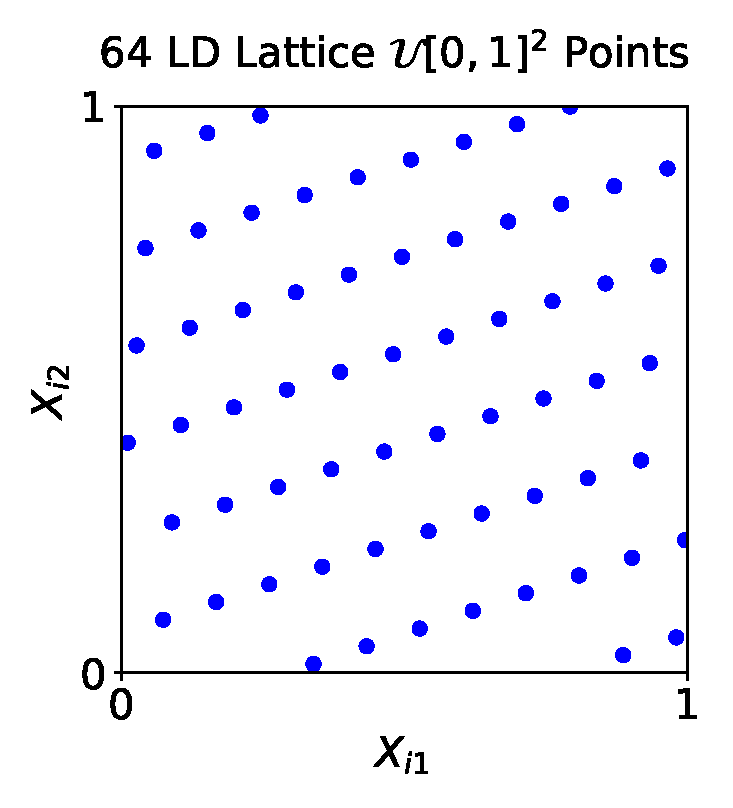
\includegraphics[width = 0.35\textwidth]{ProgramsImages/lattice_scatter.eps}
	\caption{LD lattice points, which have fewer gaps and clusters of points than either the IID or grid points. \label{fig:iid_vs_ld}}
\end{wrapfigure}

A superior approach that combines the intentional structure of a grid with the essentially dimensionless error bound or IID sampling is \hypertarget{LDlink}{ \emph{low discrepancy}} (\LD)  sampling, $\bX_1, \bX_2,  \ldots \LDSim \calu[0,1]^d$, which has an error bound of \cite{Nie92,Hic99a}
\begin{equation} \label{eq:KH}
    \hspace{-40ex} \abs{\mu - \hmu_n} \le D(\{\bX_i\}_{i=1}^n) \norm[\calf]{f - \mu}.
\end{equation}
The discrepancy,  $D(\{\bX_i\}_{i=1}^n)$, corresponds to the norm of the cubature error functional \cite{Hic97a} for the function space $\calf$.  The discrepancy is also a measure of how close the empirical distribution\footnote{The empirical distribution assigns equal probability to each point.} is close to the uniform distribution. 
The discrepancy is typically $\Order(n^{-1 + \delta})$, where $\delta$ is arbitrarily small and positive. This faster convergence rate translates into a computational cost of $\Order(\varepsilon^{-1-\delta})$ to satisfy error criterion \eqref{eq:error_crit}, under mild smoothness conditions on $f$.  The norm $\norm[\calf]{\cdot}$ is called the \emph{variation} and is a measure of function roughness.

Popular LD sampling schemes include lattices \cite{Nie92,SloJoe94,DicEtal22a} and digital nets \cite{Nie92,DicPil10a}. \cref{fig:iid_vs_ld} displays $n=64$ LD lattice points intended to mimic $\calu[0,1]^2$.  Note that a grid of $64$ points would only have $8$ different values in each coordinate direction, whereas  the LD sample covers $64$ different values in each coordinate direction.

\subsection{Stopping Criteria} \label{sec:stopcrit}
Numerical algorithms based on efficient LD sampling are commonly called \hypertarget{QMClink}{\emph{quasi-Monte Carlo}} (\QMC) algorithms. To construct a \QMC algorithm one  needs not only an LD sequence, but also reliable and practical bounds on the error $\abs{\mu - \hmu_n}$, which are    based on the function data, $f(\bX_1), f(\bX_2), \ldots$.  Such data-based error bounds inform the stopping criteria that determine a suitable sample size $n$  to satisfy  error tolerance \eqref{eq:error_crit}.

One approach is to use $N$ different randomizations of a single LD sequence to compute $N$ sample means, and then estimate the error of the grand sample mean, $\hmu_{nN} = (\hmu_n^{(1)} +  \cdots \hmu_n^{(N)})/N$, via bootstrap or the variance of these $N$ sample means.  However, finite sample theory to justify this approach is lacking, and the sample size of $nN$ may be costly.

\FH and his collaborators have developed two kinds of theoretically justified stopping criteria for LD sampling based on the Fourier coefficients of the function data, $f(\bX_1), f(\bX_2), \ldots$.  The first kind determines a bound on $\abs{\mu-\mu_n}$ by inferring the roughness of $f$ from the decay of the discrete Fourier coefficients \cite{HicJim16a,JimHic16a,HicEtal17a}.  The second kind uses  Bayesian credible intervals for $\abs{\mu-\mu_n}$ assuming that $f$ is an instance of a Gaussian process whose hyperparameters are tuned by the function data \cite{HicJag18b,RatHic19a,JagHic22a}. The cost of bounding the error $\abs{\mu-\mu_n}$ is only $\Order(n \log(n))$ for both kinds of stopping criteria.  This achieved for the Bayesian approach by choosing covariance kernels that match the LD sampling schemes, and thus avoiding the typical $\Order(n^3)$ cost.

\subsection{Software Implementation} \label{sec:software}
LD sequences are available in BRODA \cite{BRODA20a}, \MATLAB \cite{MAT9.9}, \NAG \cite{NAG27}, PyTorch \cite{paszke2019pytorch}, SciPy \cite{virtanen2020scipy}, TensorFlow \cite{tfqf2021a} and some uncertainty quantification libraries such as Dakota \cite{DakotaUsersManual}, MUQ \cite{MUQ}, UQLab \cite{UQLab2014}, and UQTk \cite{DebEtal04,UQTk}.  Efforts to identify better LD sequence generators include LatNet Builder \cite{LatNet} and the Magic Point Shop \cite{Nuy17a}.  

\FH, \YD, \SCTC, \MM, \JR, \AS and collaborators have developed more comprehensive \QMC libraries, GAIL \cite{ChoEtal21a} for \MATLAB and \QMCPy \cite{QMCPy2020a} for Python.  These libraries include the stopping criteria mentioned above, as well as flexible variable transformations of the form \eqref{eq:vartrans}.  Our recent effort is focused on \QMCPy, and includes an active repository \cite{QMCPy2020a}, documentation \cite{QMCPyDocs}, a tutorial \cite{QMCPyTutMovie2020}, and a blog \cite{QMCBlog}.


\subsection{Limitations of Existing Methodology and Software} \label{sec:limit}

There are several limitations to the methodology and software, described above, which our proposed research addresses. \cmtS{Bayesian \& big data}

\begin{description}

\item[Constructions] Identifying LD sequences, $\bX_1, \bX_2, \ldots$ require extensive offline computational work.  Furthermore, ideally they require some understanding of which coordinate directions are more significant. We address this limitation in  \cref{??} 

\item[Automatic variable transformations]  There are often multiple possible transformation $\bPsi$ that map to $\bT$ from a standard uniform random variable $\bX$ as in \eqref{eq:vartrans}.  For example, mapping $\bX \sim \calu[0,1]^d$ to $\bT \sim \caln(\bzero,\mSigma)$  involves choosing one of infinitely many possible square roots of the covariance matrix, $\mSigma$, (for $d>1$).  Choosing transformation $\bPsi$ to give an integrand $f$ with small roughness, i.e., small variation, $\norm[\calf]{f - \mu}$ is nontrivial and ideally should be based on function data. This may be addressed by adaptive importance sampling and/or  control variates. We address this limitation in \cref{??}.

\item[Multifidelity] For many practical problems, the random variable of interest $Y_\fidparam = f_\fidparam(\bX_\fidparam)$ is parameterized by a \emph{fidelity} parameter $\fidparam$, and the desired quantity of interest is $\mu_\infty = \lim_{\fidparam \to \fidparam_\infty} \bbE(Y_\fidparam)$.  For example, $f_\fidparam(\bX_\fidparam)$ may represent the numerical solution of  a partial differential equation (PDE) with random coefficients $\bX_\fidparam$ and mesh-size represented by $\fidparam$.  Typically, the cost of evaluating $Y_\fidparam$ increases with increasing fidelity, and evaluating many high fidelity $Y_{\fidparam,i}$ to approximate $\mu_\infty$ is costly.

Multifidelity (also known as multi-level or multi-index) methods \cite{Hei01a, Gil15a, HajNobTem16a} choose a sequence of fidelity parameters, $\fidparam_1, \fidparam_2, \ldots$, and write the  answer as a telescoping sum: 
\[
\mu = \mu_\infty = (\mu_{\fidparam_1} - \mu_{\fidparam_0}) + (\mu_{\fidparam_2} - \mu_{\fidparam_1}) + \cdots +
(\mu_{\fidparam_L} - \mu_{\fidparam_{L-1}}) + (\mu_{\infty} - \mu_{\fidparam_{L}}), \qquad \mu_{\fidparam_0} = 0.
\]
The sequence of fidelity parameters is chosen so that the cost of evaluating $f_{\fidparam_l}(\bX_{\fidparam_l})$  increases with $l$ (greater fidelity), but  the sample size required to estimate $\mu_{\fidparam_l} - \mu_{\fidparam_{l-1}}$ accurately decreases with $l$. The term  $\mu_{\infty} - \mu_{\fidparam_{L}}$ is approximated by zero. Substantial cost efficiency is gained by using many cheap samples to approximate the low fidelity terms and relatively fewer expensive samples to compute the high fidelity terms.  The measures of confidence or the stopping criteria mentioned in  \cref{sec:stopcrit} do not yet extend to multifidelity methods.  This is addressed in  \cref{sec:stopmulti}.

\item[More general problems than expectations] There are several problems  of interest that do not take the  form \eqref{eq:prototype}, including  computing  the quartiles of $Y$ or the (marginal) distributions of a vector random variable $\bY = \bg(\bT) = \bff(\bX)$.  The error analysis such problems is underdeveloped and the rigorous, data-based stopping criteria are non-existent. We address this limitation in  \cref{??}.

\item[Software reliability] \QMC software implemented by non-experts may be flawed.  \FH found  that randomized \PyTorch Sobol' points fell on the boundaries of $[0,1]^d$, when they never should \cite{PyTorchFirstPt2020a}.  This was due to a lack of double precision, as pointed out by \MM.  \hypertarget{LlAJRlink}{Llu\'is Antoni Jim\'enez Rugama} (\LlAJR), a former PhD student of \FH,  discovered  that \MATLAB's Sobol' sequence scrambling was incorrect.  \MATLAB corrected this after being notified.  After a vigorous discussion on the \PyTorch issues site \cite{PyTorchFirstPt2020a} and the \SciPy issues site \cite{scipySobol2020a}, \AO, \FH, and other \QMC researchers convinced the developers not to omit the first Sobol' point and to randomize by default. \AO explained why this is important~\cite{owen2020dropping}.  Unfortunately, some libraries still drop the first point of their LD sequences.  The need for a vigilant \QMC software community is addressed in  \cref{??}.


\item[Software connectivity] Solving complex problems well and efficiently may require  multiple software libraries.  For example, in uncertainty quantification, one integrand value, $f(\bX_i)$, may be the output from a PDE  library.  Not all libraries connect well, nor are there yet standards even in the QMC software community on how to pass information from one library to the next.  We address this issue in  \cref{sec:playwell}.

\end{description}


\subsection{Proposed Framework} How does our proposed framework tackle the aforementioned motivating limitations? What are specific objectives we aim to address? Should highlight QMCPy as a vessel for dissemination of our product to the broader scientific community. Should also tout our credentials in software development and collaborative experience with cutting-edge scientific \& big data applications. \cmtS{add workflow figure going from applications to tasks.}

% \subsection{Scientific Impact}
% \label{sec:sci}
% Outline the envisioned applications \& impact for the proposed framework: (Add visualization of problem)
% \begin{itemize}
% \item Physics discovery for high energy physics (Simon, with the JETSCAPE collaboration): surrogate modeling \& Bayesian inference for heavy-ion collisions
% \item Real-time control of UAVs (Simon, with UMinn collaborators): real-time control via virtual engines for unmanned aerial vehicles (big data, emulation)
% \item Bayesian optimization (Fred, Mike McCourt). Applications in food science: Simon will ping a collaborator (former student) in industry.
% \item \cmtS{Fred: random coefficients in PDE, for engineering applications.}
% \end{itemize}
% Should also talk about broader impacts of an open-source software and its impact on scientific progress. Can reiterate some of onon 4 here in the context of addressing aforementioned applications and problems.

The theoretical and methodological questions addressed by this project will include \cmtS{to modify, move later into \SEC 1? and have this has a one-paragraph abstract on the overarching framework \& broader impacts?}
\begin{enumerate}[i)]
\item Reliable adaptive importance for QMC cubature (\cref{sec:imp});
\item $\Order(n^{-3/2})$ convergence with scrambled nets for integrals over $\reals^d$ (\cref{sec:threehalves});
\item Stopping criteria for higher-order digital net (\cref{sec:HONstop}) and multilevel QMC cubatures (\cref{sec:stopML});
\item Multilevel QMC function approximation (\cref{sec:MLAppx});
\item LD subsampling for big data analytics to decrease computational cost (\cref{sec:bigdata}); and
\item LD posterior sampling methods for expensive Bayesian modeling problems (\cref{sec:bayes}).
\end{enumerate}




% %%%%%%%%%%%%%%%%%%%%%%%%%%%%%%%%%%%%%%%%%%%%%%%%%
% \section*{Overview of QMC and LD Sampling}
% %%%%%%%%%%%%%%%%%%%%%%%%%%%%%%%%%%%%%%%%%%%%%%%%%

% \cmtS{should we shorten this \& integrate as a subsection in \SEC 1?}

% %%%%%%%%%%%%%%%%%%%%%%%%%%%%%%%%%%%%%%%%%%%%%%%%%
% \subsection{Applications of (Q)MC and of IID and LD Sampling}
% %%%%%%%%%%%%%%%%%%%%%%%%%%%%%%%%%%%%%%%%%%%%%%%%%

% Many situations are best understood by mathematical models that include \emph{randomness}.  Examples include Bayesian statistical inference \cite{GelEtal13, EfrHas16}, financial risk \cite{Gla03,LEc09}, particle transport \cite{Hag14,Spa95,Vea97}, and uncertainty quantification \cite{Smi14a,HerSch20a}.  Simulations use  vectors, $\bX_1, \bX_2, \ldots$ to generate a myriad of possible outcomes, $f(\bX_1), f(\bX_2), \ldots$.  The statistical properties of these \emph{sample} outcomes---such as their means (averages)---can effectively estimate the \emph{population} quantities.  This is the (Q)MC process:  IID $\bX_i$ for simple MC and LD $\bX_i$  for QMC.

% %%%%%%%%%%%%%%%%%%%%%%%%%%%%%%%%%%%%%%%%%%%%%%%%%
% \subsection{LD Versus IID Sampling} \label{sec:LDvsIID}
% %%%%%%%%%%%%%%%%%%%%%%%%%%%%%%%%%%%%%%%%%%%%%%%%%

% \begin{flalign} \label{eq:Keister}
% \mu &= \int_{\reals^d} \cos( \norm[2]{\bt}) \exp(-\norm[2]{\bt}^2) \, \dif \bt.&
% \end{flalign}
% Under several absolute error tolerances, $\varepsilon$, QMCPy increases $n$ until \eqref{eq:error_crit} is satisfied according to the suitable stopping criteria.
% Both the number of function values and the computation time increase like $\Order(\varepsilon^{-2})$ for IID sampling and $\Order(\varepsilon^{-1-\delta})$ for LD sampling as $\varepsilon$ decreases. For $\varepsilon = 0.01$ there is a hundred-fold contrast between the $n$ and time required for IID versus LD. 

% The orders of the computational cost dependence on $\varepsilon$ for IID and LD sampling are \emph{independent of $d$}.  In contrast, tensor product rules using grid sampling satisfy \eqref{eq:error_crit} at a computational cost of $\Order(\varepsilon^{-d/r})$  if the derivatives of $f$ up to total order $rd$ exist.  Increased smoothness, $r$, helps but cannot overcome the exponential growth of the cost with $d$.

% To harness the efficiency of LD sampling, practitioners need quality, easy-to-use QMC software.  QMC researchers need a showcase  for their latest work.  QMCPy satisfies those needs. 


%%%%%%%%%%%%%%%%%%%%%%%%%%%%%%%%%%%%%%%%%%%%%%%%%
\section{A Framework for Cost-Efficient and Confident Sampling}
%%%%%%%%%%%%%%%%%%%%%%%%%%%%%%%%%%%%%%%%%%%%%%%%%

\cmtS{Need to revise \& restructure given motivating scientific \& big data aims. But topics largely OK (with a bit of expansion)?
\begin{itemize}
\item Cost-efficient Bayesian inference
\item MLQMC / Multi-level experimental design
\item Cost-efficient big data analytics
\item Cost-efficient QMC? Fred: does this capture some of the proposed topics you had here, or do we need new ideas?

\item 1) Motivation, 2) Tasks, 3) Implementation and Application
\end{itemize}
}

% QMCPy has made a good start.  Yet, much must be done to establish the critical mass of algorithms and collaborators that will make QMCPy self-sustaining. Rapid developments in science and engineering have brought about novel methodological and theoretical issues which need to be addressed, especially on expanding the scope of applicability of QMC. The subsections below highlight those research problems that we will tackle. For each problem, we indicate the primary investigators and collaborators, as well as the time periods over which they will be addressed.

% %%%%%%%%%%%%%%%%%%%%%%%%%%%%%%%%%%%%%%%%%%%%%%%%%
% \subsection{Multilevel QMC (MLQMC)} \label{sec:multilevel} [\SM lead, \FH, \YD, \PR, \IJi, \TT{}] 
% %%%%%%%%%%%%%%%%%%%%%%%%%%%%%%%%%%%%%%%%%%%%%%%%%



% %%%%%%%%%%%%%%%%%%%%%%%%%%%%%%%%%%%%%%%%%%%%%%%%%
% \subsubsection{MLQMC for Function Approximation} \label{sec:MLAppx}
% [Years 1--2]
% %%%%%%%%%%%%%%%%%%%%%%%%%%%%%%%%%%%%%%%%%%%%%%%%%
% An important extension of MLQMC is \textit{multilevel function approximation}. The set-up is as follows. Let $f: [0,1]^d \rightarrow \mathbb{R}$ be an unknown function that we wish to infer. In many problems, $f$ cannot be directly evaluated, but there are lower-accuracy (\textit{lower-fidelity}) representations of $f$ (call these $f_1, \ldots, f_L$) which can be simulated. A larger value of $l$ suggests the function $f_l$ provides a \textit{better} approximation of $f$, but also incurs a \textit{higher} cost per function evaluation. This scenario is widely encountered in physical sciences and engineering, e.g., $f_l$ can be the numerical solution of a partial differential equation (PDE) using a certain mesh of the domain, with a larger $l$ indicating a finer mesh choice for the PDE solver.

% We employ the following \textit{multilevel} approach for predicting $f$. We first evaluate the lower-fidelity functions $f_l(\cdot)$ at design points $\{\bX_i^l\}_{i=1}^{n_l}$, $l=1, \ldots L$, then use the simulated data to train a predictive model for $f(\cdot)$. We make use of the following multilevel prediction model from \cite{haaland2011accurate}:
% \begin{equation}
% \hat{f}_L(\bx) = \sum_{l=1}^L \mathcal{P}_l(\bx), \;\; \text{where $\mathcal{P}_l(\bx)$ is a predictor for \textit{refinement} $f_l(\bx) - f_{l-1}(\bx)$, $f_0 \equiv 0$.}
% \label{eq:mlpred}
% \end{equation}
% In what follows, we employ for each $\mathcal{P}_l(\bx)$ independent Gaussian process (GP) predictors \cite{santner2003design} using Mat\'ern correlations with smoothness parameter $\nu$ \cite{stein2012interpolation}. The placement of evaluation points $\{\bX_i^l\}_{i=1}^{n_l}$, $l=1, \ldots, L$ is paramount for maximizing predictive accuracy: these design points should be well spread out over $[0,1]^d$ for each level $l$, and the sample sizes $n_1, \ldots, n_L$ should be chosen to balance predictive accuracy and evaluation cost. We show next that a careful allocation of QMC points over each level allows for improved accuracy over the state-of-the-art. Related work on multilevel approximation \cite{kennedy2000predicting,haaland2011accurate,le2014recursive,le2015cokriging} deal largely with the \textit{modeling} of the multilevel predictor, but not the \textit{design} of the multilevel evaluation points, which we investigate here.

% The preliminary theorem below shows that, when the design points are selected from a QMC sequence, this multilevel predictor can achieve low approximation error with reasonable cost.
% \begin{theorem}
% Let $\varepsilon > 0$ be a desired error tolerance. Assume the \textup{bias} of $f_l$ is bounded as $\sup_{\bx \in [0,1]^d} |f_l(\bx)-f(\bx)| = \mathcal{O}(T_1^{-\alpha l})$ for some $T_1 > 1$. Further assume $C_l$, the \textup{cost} of a single evaluation of $f_l$, is bounded as $C_l = \mathcal{O}(T_2^{\beta l})$ for some $T_2 > 1$. Suppose $\{\bX_i^l\}_{i=1}^{n_l}$ are taken from a \textup{low-dispersion} QMC sequence (see \cite{niederreiter1992random,yakowitz2000global}). Then, given a cost budget of $C_\varepsilon$ and under mild regularity conditions on $f$ and $\{f_l\}_{l=1}^L$, there exists a number of levels $L$ and sample sizes $n_1, \ldots, n_L$ such that $\sup_{\bx \in [0,1]^d} |f(\bx) - \hat{f}_L(\bx)| < \varepsilon$ with total evaluation cost $C_\varepsilon = \mathcal{O}(\varepsilon^{-d/\nu})$ if $\alpha d > 2 \beta \nu$.
% \label{thm:mlqmc}
% \end{theorem}
% \noindent This theorem shows that, when the biases of the lower-fidelity functions $\{f_l (\cdot)\}_{l=1}^L$ and its evaluation costs are sufficiently bounded, a QMC sampling of design points, optimally allocated over each level, can yield the desired error tolerance $\varepsilon$ with total cost bounded by $C_\varepsilon = \mathcal{O}(\varepsilon^{-d/\nu})$. Under similar conditions, this rate on evaluation cost $C_\varepsilon$ can be shown to be faster than existing complexity rates using single-level predictors or Monte Carlo sampling \citep{wendland2004scattered}. This shows that QMC sampling is indeed effective at reducing cost complexity at a fixed error level $\varepsilon$, or equivalently, reducing approximation error given a fixed evaluation cost. This cost reduction is \textit{crucial} for a timely solution of expensive approximation problems in physical science applications (see below).

% \subsubsection*{Adaptive Sampling} While \cref{thm:mlqmc} guarantees an optimal $L$ and sample sizes $n_1, \ldots,n_L$ achieving the desired cost complexity $C_\varepsilon = \mathcal{O}(\varepsilon^{-d/\nu})$, these depend on parameters of the underlying GP models, which are unknown in practice. Thus, this optimal allocation of points needs to be determined \textit{adaptively} via sequential sampling of the lower-fidelity functions $f_l(\cdot)$. We will develop an \textit{adaptive strategy} for sequentially allocating samples $n_1, \cdots, n_L$ and a \textit{stopping rule} for determining the number of levels $L$, which provably achieves the cost complexity guarantee in \cref{thm:mlqmc}.

% \subsubsection*{Applications \& Implementation} 
% \cmtS{Discuss preliminary simulation results. Application and preliminary results in multi-fidelity modeling for heavy-ion collision emulation in JETSCAPE: we have great need for this! }

% We will demonstrate the effectiveness of this MLQMC approximation approach for a range of scientific computing problems. The PI \SM is active in multidisciplinary collaborations for nuclear physics \citep{ji2021graphical,everett2021multisystem,everett2021phenomenological,cao2021determining}, aerospace engineering \citep{mak2018efficient,yeh2018common,chang2019kernel,chang2021reduced}, and material sciences \citep{chen2020function,chen2019adaptive}, where such adaptive sampling would greatly improve predictive model building under computational budgets. We will \textit{apply this methodology for cutting-edge problems} in such applications.

% why important: in practice, want to jointly reduce error and optimize cost.

% \SMNote{
% \begin{itemize}
% \item \textit{Task 3.4.2}: \SMNote{mention curse of dimensionality: projectivity?}
% \end{itemize}
% }

% An urgently-needed yet relatively unexplored area is the use of QMC as design points for multilevel functional approximation. These approximations are widely-used as efficient surrogate models for expensive scientific computations, which can be used for scientific investigation and decision-making in a timely manner (the PI \SM has ...). \SMNote{Add related work from Karen Willcox and Max Gunzburger} \SMNote{We have a nearly-finished paper applying multilevel QMC points as designs for multi-fidelity emulators. I can add in some preliminary results on this. Arc-sin \& experimental design. Dispersion scales terribly in dimension.}

%%%%%%%%%%%%%%%%%%%%%%%%%%%%%%%%%%%%%%%%%%%%%%%%%
\subsection{Big Data Analytics} [\SM lead, \AO, \RZ, \IJi{}] \label{sec:bigdata}
%%%%%%%%%%%%%%%%%%%%%%%%%%%%%%%%%%%%%%%%%%%%%%%%%

%%%%%%%%%%%%%%%%%%%%%%%%%%%%%%%%%%%%%%%%%%%%%%%%%
\subsubsection{Motivation and Preliminary Results} 
%%%%%%%%%%%%%%%%%%%%%%%%%%%%%%%%%%%%%%%%%%%%%%%%%
Big data is ubiquitous with recent advances in technology and computing power. A key challenge is that learning algorithms need to be highly \textit{efficient} and \textit{scalable} to extract information for real-time decision-making. One strategy is to iteratively train the model on small batches of the data, typically sampled uniformly at random. This \textit{subsampling} is used to scale up powerful state-of-the-art machine learning algorithms, such as stochastic gradient descent (SGD, \cite{Bot2010}) and stochastic gradient boosting \cite{friedman2002stochastic}.

\sloppypar Consider SGD, which minimizes the loss $L(\theta;\mathcal{X}) = N^{-1} \sum_{m=1}^N l(\theta;\bX_m)$ over model parameters $\theta \in \mathbb{R}^q$, where $\mathcal{X} = \{\bX_m\}_{m=1}^N \subset \mathbb{R}^d$ is the big training data (the sample size $N$ can be on the order of billions, see PI \SM's work \cite{mak2018efficient}). Standard gradient descent methods \cite{nocedal2006numerical} are impractical here, since they require evaluation of the full gradient $N^{-1} \sum_{m=1}^N \nabla_\theta l(\theta;\bX_m)$, which is very expensive with $N$ large. Mini-batch SGD \cite{Bot2010} approximates this via a subsample $\mathcal{X}_{s}^{[l]} \subset \mathcal{X}$ of size $n \ll N$, taken IID and uniformly from big data $\mathcal{X}$. The descent steps are then iterated until convergence:
\begin{equation}\label{eq:sgdopt}
\theta^{[l+1]} \leftarrow \theta^{[l]} - \eta \Biggl( \frac{1}{n} \sum_{\bX \in \mathcal{X}_{s}^{[l]}} l(\theta;\bX)\Biggr) , \quad l = 1, 2, \ldots,
\end{equation}
where $\eta$ is the gradient descent step size. Mini-batch SGD is widely used for scalable training of neural networks and deep learning models with big data \citep{srivastava2014dropout}.

Mini-batch SGD has a key limitation: since gradients are estimated by \textit{random} subsampling, the solution sequence $(\theta^{[l]})_{l=1}^\infty$ converges to a \textit{noise ball} of radius $\mathcal{O}(n^{-1})$ around the global optimum $\theta^*$. For small subsample sizes $n$, SGD can thus return estimates
\textit{very far} from  $\theta^*$. Our solution is to carefully choose an LD dataset that well-represents the big data $\mathcal{X}$. This is known as ``data squashing'' (termed by \AO in \cite{owen2003data}), and encompasses recent work on leverage-score subsampling \cite{ma2015statistical}, coresets \cite{chan2006faster,bachem2017practical, huggins2016coresets}, and work by PI \SM \cite{mak2018support,mak2018minimax,mak2017projected,krishna2019distributional}. The problem of LD data squashing for large-scale SGD, however, is timely and challenging, but largely unaddressed in the literature.
% Existing methods, however, do not apply directly for the problem of data squashing for SGD optimization.

We propose a new data squashing method which makes use of a LD subsample of big data $\mathcal{X}$ for accelerating SGD. The preliminary result below guarantees the \textit{existence} of such a subsample:
\begin{theorem}
Let $\mathcal{X} = \{\bX_m\}_{m=1}^N$ (the ``big data'') be any set of points on $[0,1]^d$, and suppose the feasible space $\Theta$ is convex. Further suppose $n \leq \sqrt{N}$ and the loss function $l$ is convex with mild regularity conditions. Then there exists a subsample $\mathcal{X}_s \subseteq \mathcal{X}$ of size $n$ which, when used within the SGD iterative updates \eqref{eq:sgdopt}, yields a solution sequence $(\theta^{[l]})_{l=1}^\infty$ converging to a noise ball of radius $\mathcal{O}\{(\log n)^{3d+1}/n^2\}$ around the global optimum $\theta^*$.
\label{thm:ldsgd}
\end{theorem}
\noindent This theorem guarantees that, under mild assumptions on the loss function $l$, there exists an LD subsample of the big data which, when used within SGD, converges a noise ball of radius $\mathcal{O}\{(\log n)^{3d+1}/n^2\}$ around the desired solution $\theta^*$. Thus, with a carefully chosen LD subsample, the proposed ``LD-batch SGD'' can yield \textit{improved} optimization over standard mini-batch SGD, which converges to a \textit{larger} noise ball of radius $\mathcal{O}(n^{-1})$. Put another way, this suggests that LD-batch SGD can yield comparable performance to mini-batch SGD with far fewer optimization iterations, thereby providing \textit{large computational savings for big data analysis}.

We will tackle the following tasks to flesh out a comprehensive methodological framework for LD-batch SGD, implementable within QMCPy.


%%%%%%%%%%%%%%%%%%%%%%%%%%%%%%%%%%%%%%%%%%%%%%%%%
\subsubsection{Optimization for LD-batch SGD} [Years 1--2]
%%%%%%%%%%%%%%%%%%%%%%%%%%%%%%%%%%%%%%%%%%%%%%%%%
While the existence of an LD subsample is promising, one challenge is in finding such a subset efficiently. We will find this via the following optimization approach. Define the so-called ``data kernel'' using the big data $\mathcal{X} = \{\bX_m\}_{m=1}^N$:
\begin{equation}
K_{\rm data}(\bx,\by) = \sum_{\bk \in \mathbb{Z}^d \setminus \mathbf{0}} \lambda_{\bk} \phi_{\bk}(\bx)\overline{\phi_{\bk}(\by)}, \quad \phi_{\bk}(\bx) = e^{2 \pi {\rm i} \bk^T\bx} - b_{\bk}, \quad b_{\bk} = \frac{1}{N} \sum_{m=1}^N e^{2 \pi {\rm i} \bk^T\bX_m}.
\end{equation}
where ${\rm i}$ is the imaginary number, and $\lambda_{\bk}=\prod_{j=1}^d \max(1,2\pi|k_j|)^{-2}$. Here, the coefficients $b_{\bk}$ can be efficiently computed via non-linear fast Fourier transform \citep{wahls2015fast}. The data kernel $K_{\rm data}$ has two nice properties. We can show that the subsample $\mathcal{X}_s$ minimizing the kernel discrepancy with $K_{\rm data}$ yields the improved rate in \cref{thm:ldsgd}. We can also show that, with all coefficients computed, this discrepancy can be evaluated in $\mathcal{O}(n^2)$ work, \textit{independent} of $N$ (the big data size). We will develop \textit{scalable algorithms to optimize this data discrepancy for LD subsampling}, leveraging recent developments in accelerated gradient descent \citep{jin2018accelerated} and randomized algorithms \citep{mahoney2011randomized}.

%%%%%%%%%%%%%%%%%%%%%%%%%%%%%%%%%%%%%%%%%%%%%%%%%
\subsubsection{Application and Implementation}
[Years 2--3]
%%%%%%%%%%%%%%%%%%%%%%%%%%%%%%%%%%%%%%%%%%%%%%%%%

\cmtS{Discuss UAV application with preliminary results, where we're trying to build emulators for real-time control via virtual engines (digital twins). We need these virtual engines (with emulators) to provide robust and real-time control in milliseconds. There are $n \approx 25,000$ data points for curve emulation, and we need to achieve this quickly. Some preliminary results.}

\cmtS{move later} We will provide an efficient and streamlined implementation of LD-batch SGD within QMCPy. Given recent breakthroughs in high-performance and distributed computing, we will develop scalable algorithms which exploit such technologies for efficient LD-batch subsampling. We will also provide specific \textit{implementations} of LD-batch SGD for \textit{popular learning models} (e.g., regression, neural networks, kernel methods) on QMCPy.

% \textit{We will implement these existing methods} in QMCPy, and explore their effectiveness in a suite of big data problems. There is little work on which data squashing procedure is most appropriate for SGD optimization. Our preliminary results show that a LD subsample exists for \textit{any} big dataset $\mathcal{X} \subset \mathbb{R}^d$ that achieves a noise ball radius of $\mathcal{O}\{(\log n)^{3d+1}/n^2\}$. We will investigate this further and implement this in QMCPy.

%%%%%%%%%%%%%%%%%%%%%%%%%%%%%%%%%%%%%%%%%%%%%%%%%
\subsection{Expensive Bayesian Modeling} [\SM lead, \FH, \YD, \TT{}] \label{sec:bayes}
%%%%%%%%%%%%%%%%%%%%%%%%%%%%%%%%%%%%%%%%%%%%%%%%%

%%%%%%%%%%%%%%%%%%%%%%%%%%%%%%%%%%%%%%%%%%%%%%%%%
\subsubsection{Motivation and Preliminary Results}
%%%%%%%%%%%%%%%%%%%%%%%%%%%%%%%%%%%%%%%%%%%%%%%%%
Bayesian methods have become popular in recent decades, primarily due to their ability to fit complex models via sampling \cite{GelEtal13}. Such methods rely on MCMC sampling for exploration of the posterior distribution $F$, which captures information on model parameters. However, with the rise of big data and complex learning models, the posterior $F$ is often \textit{expensive} to evaluate, thus making MCMC sampling very \textit{time-consuming} \cite{joseph2015sequential}. This is compounded by the highly correlated nature of MCMC samples, which reduces the information provided by each sample \citep{link2012thinning}. For such expensive Bayesian problems, an LD posterior sampling method can \textit{greatly improve model learning given a computational budget}.

% While the QMC Metropolis method by \cite{OweTri05a} speeds up the convergence of samples, it still requires many posterior evaluations. We want method which can provide LD sampling with limited posterior evaluations here.

One approach for LD posterior sampling is to minimize the \textit{kernel discrepancy} $D_K(\{\bX_i\}_{i=1}^n, F)$ \cite{Hic99a}, which measures the difference between the empirical distribution of $\{\bX_i\}_{i=1}^n$ and the posterior $F$ via a symmetric, positive-definite kernel $K$. This is known as \textit{kernel herding} \citep{chen2012super}. Kernel herding has a key limitation: this discrepancy requires an analytic form for the integral $\int K(t,\bX) \, \dif F(t)$, which is unattainable for complex posteriors $F$. To address this, \cite{chen2018stein} proposed the \textit{Steinized kernel}:
\begin{multline}\label{eq:stein}
K_{\rm ST}(\bt,\bx) = \nabla_\bt \cdot \nabla_\bx K(\bt,\bx) + \nabla_\bt K(\bt,\bx) \cdot \nabla_\bx \log \dif F(\bx)\\
 + \nabla_\bx K(\bt,\bx) \nabla_\bt \log \dif F(\bt) + K(\bt,\bx) \nabla_\bt \log \dif F(\bt) \cdot \nabla_\bx \log \dif F(\bx),
\end{multline}
where $\nabla$ and $\nabla \cdot$ are the gradient and divergence operators. The key advantage is that the integral in question, $\int K_{\rm ST}(t,\bX) \, \dif F(t)$, evaluates to 0 for all $\bX$, thus allowing one to generate LD posterior samples via direct discrepancy minimization. With this closed-form $D_K(\{\bX_i\}_{i=1}^n, F)$ with kernel $K=K_{\rm ST}$, \cite{chen2018stein} employ a sequential optimization procedure: the first sample $\bX_1^*$ is taken at the \textit{mode} of $F$, then subsequent samples $\bX_2^*, \bX_3^*, \cdots$ are obtained by sequentially optimizing $D_K(\{\bX_i\}_{i=1}^n, F)$. The optimized samples $\{\bX_i^*\}_{i=1}^n$, called \textit{Stein points}, gives improved representation of the posterior $F$ over standard MCMC methods, thereby providing significant computation savings for learning complex Bayesian models.

Despite this, Stein points have a key limitation: they do not provide \textit{inference} for computed posterior quantities. Suppose we estimate the posterior mean $\mu = \mathbb{E}_{\bX\sim F}[g(\bX)]$ with $\hat{\mu}_n = n^{-1}\sum_{i=1}^n g(\bX_i^*)$, where $\{\bX_i^*\}_{i=1}^n$ are the Stein points. With these \textit{deterministic} samples, it is difficult to infer the error $|\mu - \hat{\mu}_n|$, since the deterministic error bounds for Stein points (see \cite{chen2018stein}) contain many constants which cannot be estimated in Bayesian problems. But the quantification of estimate uncertainty is paramount for expensive Bayesian problems: it provides a principled way to assess whether the posterior sample taken is large enough for validating scientific findings.

We propose a novel \textit{Randomized Stein points} (RSPs) method which addresses this need. This idea is inspired by randomized lattice rules (see \cite{l2002recent}), which randomizes lattices on $[0,1]^d$ by randomly shifting its first point. Here, instead of taking the first sample $\bX_1^*$ at the \textit{mode} of $F$, we select this point  \textit{randomly} from $F$ (e.g., after an initial MCMC burn-in). Subsequent samples $\bX_2^*, \bX_3^*, \cdots$ are then obtained via sequential optimization of $D(\{\bX_i\}_{i=1}^n, F)$, similar to the original Stein points. This random initialization for RSPs allows for probabilistic inference on error $|\mu - \hat{\mu}_n|$. Since the samples $\{\bX_i^*\}_{i=1}^n$ are now \textit{random}, one can now apply probabilistic confidence intervals used for standard MCMC samplers (e.g., \cite{atchade2016markov,rosenthal2017simple}). \cref{fig:rsp} compares the performance of RSPs with two popular MCMC samplers: Random-Walk Metropolis (RWM, \cite{metropolis1953equation}) and the Metropolis-Adjusted Langevin Algorithm (MALA, \cite{roberts1996exponential}), for a simple 1-d mixture normal distribution $F$. The left plot shows the effective sample size (ESS, a measure of sample quality \cite{GelEtal13}) of $n=300$ samples, and the right plot shows the length and coverage ratio of a simple 95\% confidence interval (CI) $\hat{\mu}_n \pm 1.96 \hat{\sigma} / \sqrt{\text{ESS}}$ for the mean of $F$, where $\hat{\sigma}^2$ is the estimated variance of the integrand. We see that RSPs enjoy noticeably improved sample quality (higher ESS), which translates to more precise CIs (smaller CI length) and higher coverage ratios. This suggests the proposed RSPs indeed provide the improved sample efficiency and uncertainty quantification required for expensive Bayesian problems.

\begin{wrapfigure}{r}{0.45\textwidth}
	\centering
	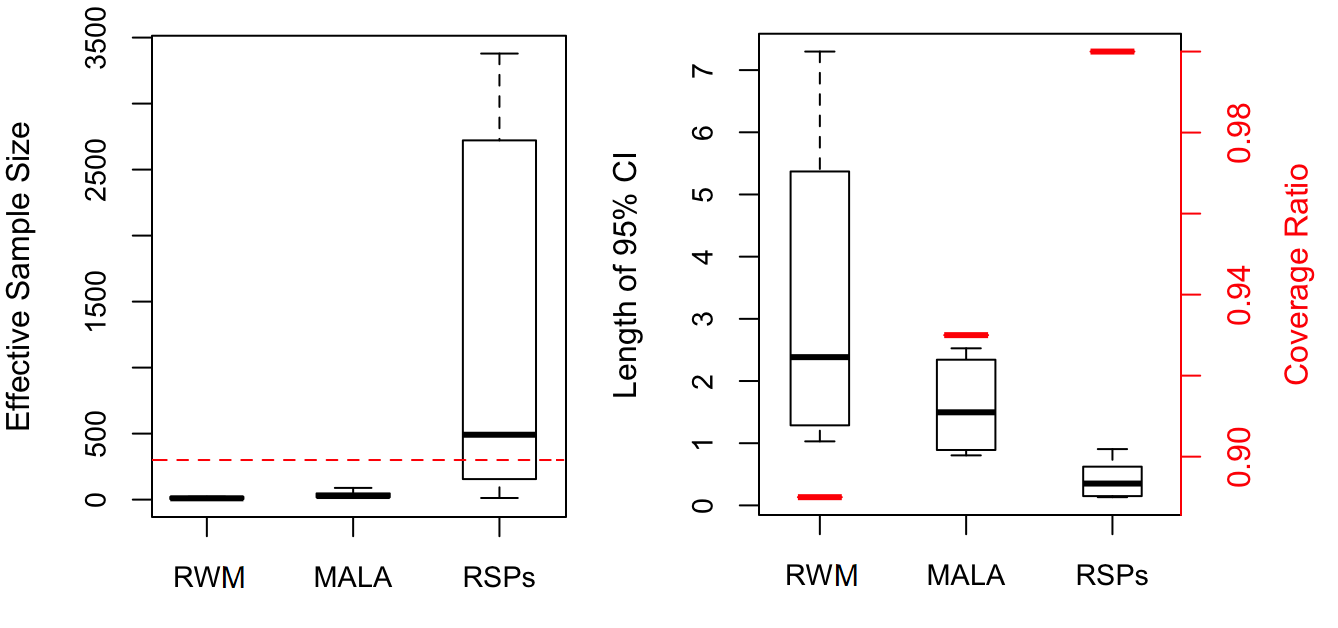
\includegraphics[width = 0.45\textwidth] {ProgramsImages/rsp.png}
	\caption{ESS (left) and CI length / coverage ratio (right) for $n=300$ samples using RMW, MALA and RSPs. Boxplots show the distribution of metrics over 100 simulation replications. \label{fig:rsp}}
	\vspace{-0.6cm}
\end{wrapfigure}

We will tackle the following tasks to develop RSPs for efficient Bayesian learning in QMCPy.
%%%%%%%%%%%%%%%%%%%%%%%%%%%%%%%%%%%%%%%%%%%%%%%%%
\subsubsection{Theory} [Years 1--3]
%%%%%%%%%%%%%%%%%%%%%%%%%%%%%%%%%%%%%%%%%%%%%%%%%
We will investigate key theoretical properties for RSP sampling. One property to show is that the subsequent RSP samples $\bX_2, \bX_3, \ldots$, which are \textit{random} due to the randomness of $\bX_1$, indeed follow (or closely approximate) the posterior distribution $F$. Another property to prove is a Central Limit Theorem which characterizes the asymptotic distribution of error $|\mu-\hat{\mu}_n|$ as $n \rightarrow \infty$. This is crucial for not only verifying the asymptotic correctness of the RSP CIs (see \cite{rosenthal2017simple}), but also demonstrating improved convergence over standard MCMC samplers.

%%%%%%%%%%%%%%%%%%%%%%%%%%%%%%%%%%%%%%%%%%%%%%%%%
\subsubsection{Applications \& Implementation} [Years 2--3] 
%%%%%%%%%%%%%%%%%%%%%%%%%%%%%%%%%%%%%%%%%%%%%%%%%
\cmtS{Discuss preliminary simulation results and ball dropping toy application. Application for turbomachinery application, where we can pull out gradients from our simulators. }


% \SMNote{expand on novel developments} \textit{We will implement Stein points} in QMCPy. PI \SM has worked on a variety of complex Bayesian modeling problems, from climatology \cite{mak2016regional} to aerospace engineering \cite{mak2018efficient,chang2019kernel,yeh2018common}, and we will explore the effectiveness of Stein points for such problems. We will also explore further extensions of Stein points for approximate Bayesian computation, a popular class of Bayesian methods for population genetics and epidemiology.



%%%%%%%%%%%%%%%%%%%%%%%%%%%%%%%%%%%%%%%%%%%%%%%%%
\subsection{Adaptive Algorithms for Multifidelity Problems} [\FH lead, \SCTC, \YD, \MM, \DN, \CH, \AO, \AS{}] \label{sec:performance}
%%%%%%%%%%%%%%%%%%%%%%%%%%%%%%%%%%%%%%%%%%%%%%%%%
\cmtS{ideas on gauging confidence, adaptive algorithms, uncertainty quantification.} \cmtS{structure: Motivation \& preliminary results, Action tasks, Application \& implementation?}

\subsubsection{Motivation and Preliminary Results} A common form of uncertainty quantification involves computing $\mu = \bbE(Y)$, where $Y=f(\bX)$ and $f$ can only be approximated by $f_\fidparam$, where $\fidparam$ denotes the fidelity of the approximation.  E.g., $f$ is the solution of a (partial) differential equation whose coefficients and/or boundary conditions are given by a random field, and $\fidparam$ denotes the mesh size of the numerical solver and the discretization of the random field.  

As mentioned in \cref{sec:limit}, approximating the true solution, by a single high fidelity expectation is costly.  Rather, multifidelity methods \cite{Hei01a, Gil15a, HajNobTem16a}---the object of active research---consider a sequence of problems, $\{\mu_l =\bbE[f_{\fidparam_l}(\bX_{\fidparam_l})] \}_{l=0}^L$, where the fidelity increases with $l$ as does the computational cost of evaluating an instance $f_{\fidparam_l}(\bX_{\fidparam_l,i})$.  One can efficiently approximate $\mu$ by using more cheap samples to approximate $\mu_l - \mu_{l-1}$ for small $l$ and fewer  expensive samples to approximate $\mu_l - \mu_{l-1}$ for large $l$.

\subsubsection{Extending Stopping Rules to Multifidelity Problems}\label{sec:stopmulti} [Years 1-2]
Adaptive algorithms for these multifidelity problems use ad hoc stopping criteria.  We propose to develop  rigorous stopping criteria like those described in \cref{sec:stopcrit}.   \FH, \AS,  \JR, and collaborators have  developed stopping criteria for functions of several expectations, $C(\bmu)$, \cite{HicEtal17a, JagSor23a}.  For example, Bayesian posterior means, \cite{GelEtal13}, can be written as the ratio of two  expectations, $C(\bmu) = \mu_2/\mu_1$.  Sensitivity indices \cite{Sob01,Sal02a,SalEtal08a} also involve the  computation of more than one expectation.  However, in both these cases, the underlying random vector, $\bX$, is the same for all expectations, $\mu_1, \,mu_2, \dots$, and only the functions $f_l$ defining the expectations are different.

For multifidelity problems each $\mu_l$ depends on a different $\bX_{\fidparam_l} \sim \calu[0,1]^{d_l}$ with a different $d_l$.   Thus, adaptive algorithms need to manage LD sequences of different dimensions as well as different sample sizes.  Adaptive decisions must be made on whether to devote more effort to sampling the low fidelity or high fidelity terms.  The wealth of literature in on multifidelity methods and our experience on developing rigorous stopping criteria for single fidelity problems gives us confidence in success.

\subsubsection{Variance/Variation Reduction Through Importance Sampling} \label{sec:imp} %%%%%%%%%%%%%%%%%%%%%%%%%%%%%%%%%%%%%%%%%%%%%%%%%
[Years 1--3]  The discrepancy \eqref{eq:KH} measures the difference between the empirical distribution of the sampling sites and the uniform distribution.  In many cases, the original problem is posed as an integral over $\reals^d$, as on the left side of \eqref{eq:imp}, and a variable transformation must be performed to obtain an integral over $[0,1]^d$.  Note that $f_{\bT}(\bx) = g(\bT(\bx)) \lambda(\bT(\bx)) / \varrho(\bT(\bx))$, where $\varrho$ is the density of $\bT(\bX)$ with $\bX \sim \calu[0,1]^d$.  While in some cases one may choose $\bT$ such that $\varrho(\bt) = \lambda(\bt)$, this is not the only choice and may not be the best choice.  Choosing the transformation $\bT$ is equivalent to performing importance sampling.   

The Koksma-Hlawka inequality, \eqref{eq:KH}, tells us to choose $\bT$ to make the variation, $\norm[\calf]{f_{\bT} - \mu}$, small.  For randomized QMC we want to make the variance of $\hmu_n$ small.  Intuitively, variance/variation reduction is making $f_{\bT}$ as flat as possible. As illustrated in the Keister example \eqref{eq:KeisterAlt}, finding a better $f_{\bT}$ may significantly reduce the computation time.  We will \emph{implement adaptive importance sampling}, drawing on the work of  
\AO \cite{owen2000safe} for safe importance sampling, the  annealed importance sampler \cite{neal2001annealed}, and the bridge sampler \cite{gelman1998simulating}.  Recent work includes \cite{mueller2019neural}, which uses deep neural networks for importance sampling in image rendering.  In \cite{huling2020energy}, PI \SM extends importance sampling for covariate balancing in causal inference.  \FH's PhD student, \KZ, has shown how importance sampling with QMC can beat MCMC in computing the posterior means of logistic regression coefficients \cite{Zha21a}.  We will determine \emph{theoretically and empirically} under what conditions adaptive importance sampling makes \emph{significant improvement in computation times.}

%%%%%%%%%%%%%%%%%%%%%%%%%%%%%%%%%%%%%%%%%%%%%%%%%
\subsubsection{Attaining $\Order(n^{-3/2})$ Convergence for Scrambled Nets} \label{sec:threehalves}
%%%%%%%%%%%%%%%%%%%%%%%%%%%%%%%%%%%%%%%%%%%%%%%%%
[Years 2--3] \AO showed that for moderately smooth integrands, $f$, integrated over the unit cube, the RMSE using randomly scrambled digital nets is $\Order(n^{-3/2})$ \cite{Owe97}.  \FH and collaborators extended this work \cite{HicYue00,HeiHicYue02a}.  However, this convergence rate does not always hold up when the original integrand is over $\reals^d$ because the natural transformation, $\bT$,  in \eqref{eq:imp} and \cref{sec:imp} introduces singularities into $f_{\bT}$.

Consider the following two integrals:
\begin{equation} \label{eq:getthreehalves}
	\mu_1 = \int_{[0,1]^3} g(\bt) \, \dif \bt, \quad \mu_2 = \int_{\reals^3} g(\bt) \phi(\bt) \, \dif \bt, \qquad \text{where } g(\bt) = \exp(t_1 + 0.0625 t_2 + 0.0123t_3), 
\end{equation}
\begin{wrapfigure}{r}{0.65\textwidth}
	\centering
	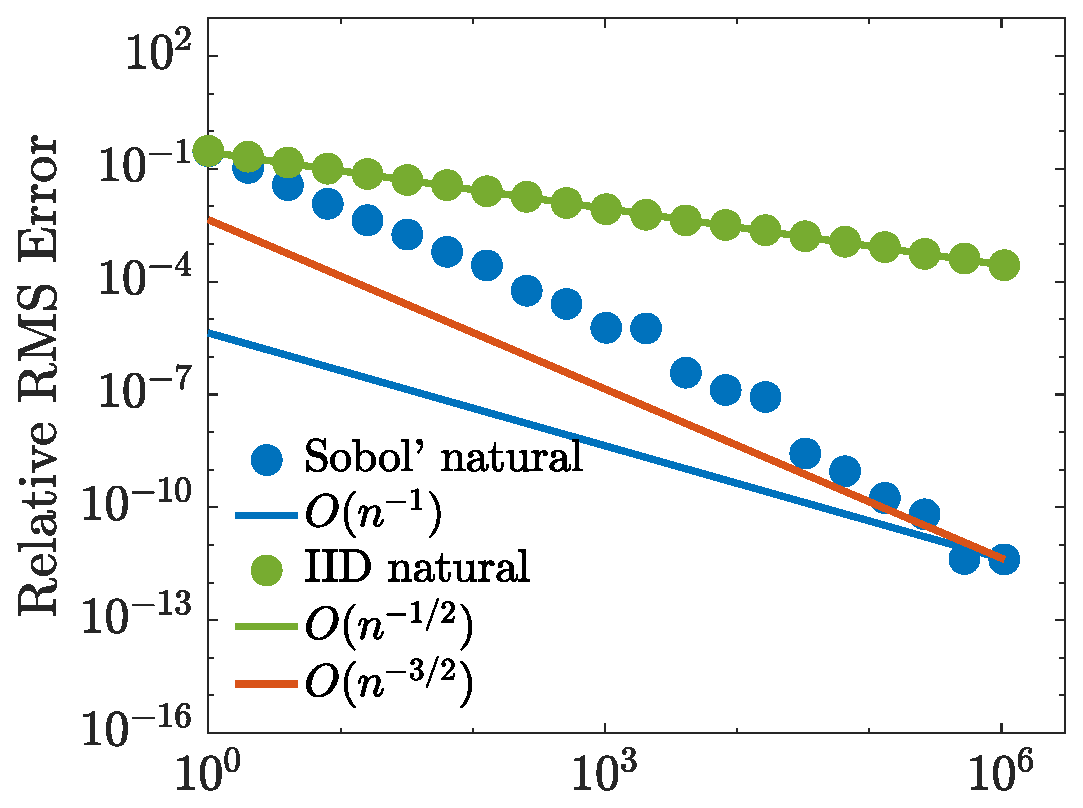
\includegraphics[width = 0.32\textwidth] {ProgramsImages/ConvergeRateStrat_exp_uniform_natural_d3_m20.eps}
	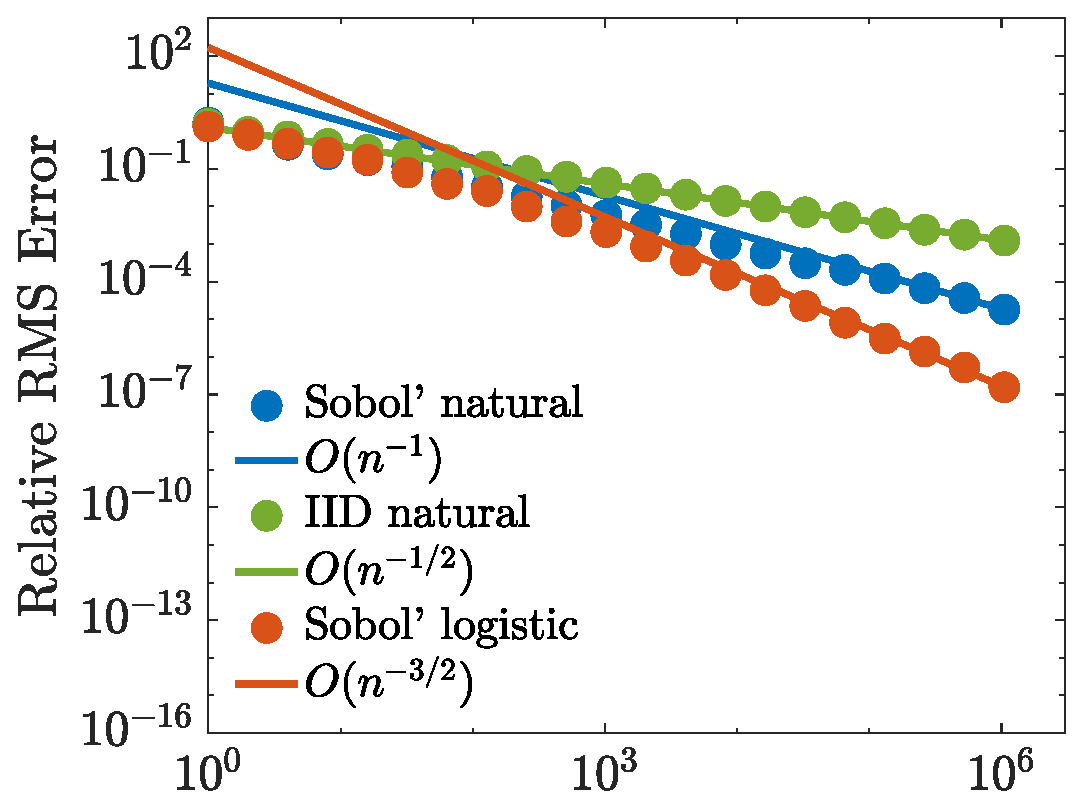
\includegraphics[width = 0.32\textwidth] {ProgramsImages/ConvergeRateStrat_exp_stdGauss_logistic_d3_m20.eps}
	\caption{The relative RMSE  for scrambled Sobol' cubature for integrals $\mu_1$ (left) and $\mu_2$ (right) defined in \eqref{eq:getthreehalves}.  For $\mu_1$ the natural transformation of $\bT(\bx) = \bx$ yields the expected $\Order(n^{-3/2})$ error, whereas for $\mu_2$ the natural inverse normal distribution function transformation, yields only $\Order(n^{-1})$  error. \label{fig:obtainthreehalf}}
\end{wrapfigure}
where $\phi$ is the standard trivariate normal density.  IID cubature for $\mu_1$ and $\mu_2$ yields an RMSE of $\Order(n^{-1/2})$ as shown in \cref{fig:obtainthreehalf}.  For $\mu_1$, scrambled Sobol' cubature yields an $\Order(n^{-3/2})$ RMSE.  However, for $\mu_2$, the natural transformation of variables, corresponding to the inverse distribution function, gives only $\Order(n^{-1})$ RMSE.  Importance sampling with the heavier tailed logistic distribution reclaims the desired $\Order(n^{-3/2})$ error.  

It is not clear how to obtain $\Order(n^{-3/2})$ error using scrambled net cubature for integrals of the form $\mu_2$ and \emph{general} $g$ and dimension, $d$.  We will return to the original work cited above that proves $\Order(n^{-3/2})$ error for integrals of the form $\mu_1$, and \emph{extend this theory to integrals of the form $\mu_2$.}  Prudent importance sampling seems necessary.

%%%%%%%%%%%%%%%%%%%%%%%%%%%%%%%%%%%%%%%%%%%%%%%%%
\subsubsection{Stopping Criteria for Higher Order Net Cubature} \label{sec:HONstop} 
%%%%%%%%%%%%%%%%%%%%%%%%%%%%%%%%%%%%%%%%%%%%%%%%%
[Years 2--3] Josef Dick introduced the concept of higher order nets, and showed how these give $\Order(n^{-\alpha})$ convergence rates for QMC cubature, where $\alpha$ reflects the smoothness of the integrand and the order of the net \cite{Dic08a,Dic09a,Dic11a}.  The stopping criteria developed by PI \FH and his collaborators \cite{HicJim16a,HicEtal17a,Jag19a}, are not designed for these higher order nets because they only track the decay of the Walsh coefficients of the integrand. We will \emph{develop stopping criteria for higher order net cubature}, by extending \cite{HicJim16a} in tracking a more nuanced measure of these fast Walsh coefficients that matches the definition of higher order nets.  We will extend the Bayesian stopping criterion in \cite{Jag19a} by identifying smoother digital shift invariant covariance kernels whose Gram matrices can be decomposed by a fast Walsh transform.



%%%%%%%%%%%%%%%%%%%%%%%%%%%%%%%%%%%%%%%%%%%%%%%%%
\subsubsection{Connecting with Other Libraries} [Years 1--2] \label{sec:playwell}
%%%%%%%%%%%%%%%%%%%%%%%%%%%%%%%%%%%%%%%%%%%%%%%%%
The complex multifidelity problems that we want to solve will often receive $f_{\fidparam}(\bX_{\fidparam})$ as the output of another library.  We will work with popular library developers to provide demos that show  how our \QMCPy library connects with theirs.  We recently collaborated with Uncertainty Quantification and Model Bridge (UM-Bridge) effort \cite{umbridge} to make \QMCPy compatible with UM-Bridge.

We will also connect QMCPy to other libraries such as PyTorch \cite{paszke2019pytorch}, SciPy \cite{virtanen2020scipy}, TensorFlow \cite{tfqf2021a}, taking advantage of what they offer in \QMCPy and pushing our more widely accepted developments into them.  A recent lunch gathering at an international \QMC conference initiated by \FH raised the need to standardize formats for LD generators to allow them to be shared across software libraries.  We will pursue this and other initiatives that promote same look-and-feel across \QMC software.



%%%%%%%%%%%%%%%%%%%%%%%%%%%%%%%%%%%%%%%%%%%%%%%%%
\subsection{Adaptive Algorithms for Quantile and Distribution Estimation} [\FH lead, \AO, \AS{}]
%%%%%%%%%%%%%%%%%%%%%%%%%%%%%%%%%%%%%%%%%%%%%%%%%

%%%%%%%%%%%%%%%%%%%%%%%%%%%%%%%%%%%%%%%%%%%%%%%%%

\subsubsection{Motivation and Preliminary Results}

\cite{AbdEtal21a}




\section{Broader Impacts}

% \cmtS{``Broader Impacts and Implementation''? We can then discuss QMCPy as an open-source vessel for disseminating the proposed framework, geared towards the goal of scientific progress \& engineering advancement, etc.}

\subsection{Disseminating Our Work} We will publish our theoretical and practical work in a variety of mathematics, statistics, and computer science journals and conference proceedings. We will present our work at conferences targeting theoreticians and practitioners.  We will offer tutorials.  Students will present at conferences and during group meetings, as part of their education. \cmtS{expand and discuss cross-disciplinary dissemination to the broad scientific community? some sample writing below from another proposal}

\subsection*{Dissemination to the Broad Scientific Community}
In order for SCINPL to be an integral component in solving modern complex scientific problems, scientists need to be convinced that our modeling paradigm can faithfully represent useful scientific information as prior beliefs, and can provide models which are not only data-efficient, but also scientifically interpretable and meaningful for the problem at hand. This necessitates a \textit{strategic outreach} and \textit{targeted dissemination} of the proposed methodologies to a broad range of scientific communities, who may not be familiar with statistical modeling. We will achieve this outreach in two key ways: a multi-disciplinary publication plan for research dissemination, and an open-source software implementation plan. 

Our publication plan will target a broad multi-disciplinary audience. We will publish our work in not only statistics, machine learning, and mathematics journals, but will also top subject-matter journals to make the proposed tools accessible and approachable to the scientific community. We will post all our work as freely accessible papers on arXiv, with links to open source and well documented code on GitHub to allow for easier dissemination of our methods to end-users. We will also give talks, tutorials and workshops at prominent statistics, machine learning, and scientific conferences, educating different communities on promising developments and exciting breakthroughs in science-integrated statistical learning.


\subsection{QMCPy as a Proving Ground} \label{sec:provingground}
\cmtS{Fred \& Yuhan: maybe shorten the writing below, and focus on QMCPy as a vessel for connecting our new methods (\& existing state-of-the-art) to scientific practitioners who will use such tools for cost-efficient solutions to cutting-edge scientific problems.} QMCPy will aggregate the best QMC software with a clear structure and a consistent user interface.  When a potentially better LD generator, algorithm, or use case arises, it will be simple to swap out the old for the new and measure performance while all other pieces remain the same.  Moreover, the theoretical developments will pave the way for QMC in new application areas.

QMCPy will \emph{stand in the breach} between research code from individual groups and large-scale software packages.  Research groups need to compare their new ideas with the best available.  Those who develop LD generators need to test them on a variety of use cases and as key components of various QMC algorithms.  Those with new QMC algorithms need to test them with the best generators.  Those with juicy use cases want to try the best that QMC offers.  Because large-scale software packages like \SciPy, \PyTorch, \TensorFlow, \NAG, or \MATLAB, do not offer QMCPy's options,  QMCPy \emph{will attract a significant number of QMC researchers as contributors.}

Although large-scale software packages cannot adopt every new QMCPy wrinkle, QMCPy algorithms attracting broad interest will be folded into these large-scale packages. \MATLAB adopted \FH's TOMS LD generators from \cite{HonHic00a}. As a library that strives to connect the best of QMC software to the scientific community, the success of QMCPy will be gauged by how well such a connection is made. We will thus measure project success via a variety of \emph{engagement} metrics (e.g., number of package downloads, GitHub pull requests), as well as the degree of integration into large-scale packages.  A recent conference special session including the QMC developers for \SciPy, \PyTorch, and \TensorFlow has already opened dialogue on further collaboration.

%%%%%%%%%%%%%%%%%%%%%%%%%%%%%%%%%%%%%%%%%%%%%%%%%
\subsection*{The Start of QMCPy}
%%%%%%%%%%%%%%%%%%%%%%%%%%%%%%%%%%%%%%%%%%%%%%%%%

\begin{wrapfigure}{r}{0.35\textwidth}
	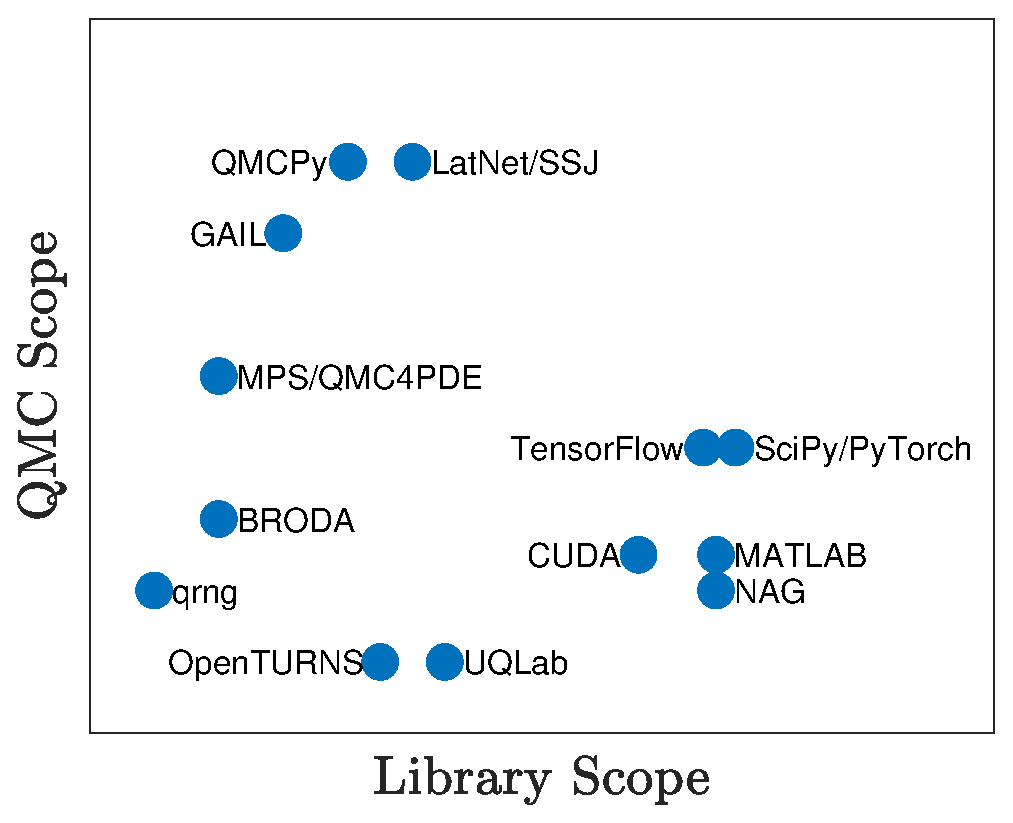
\includegraphics[width = 0.34\textwidth]{ProgramsImages/QMCSoftwarePlot.eps}
	\caption{A comparison of the scopes of libraries containing QMC software.  Some libraries with broad scope have limited QMC coverage, and vice versa.}
	\vspace{-0.3cm}
\end{wrapfigure}

\sloppypar The better existing QMC software packages include
BRODA \cite{BRODA20a}, GAIL by \FH, \SCTC, \YD, and collaborators \cite{ChoEtal21a}, LatNet Builder \cite{LatNet} and Stochastic Simulation in Java (SSJ) \cite{SSJ}, \MATLAB \cite{MAT9.10}, NAG \cite{NAG27}, multilevel (Quasi-)Monte Carlo routines  by Giles \cite{GilesSoft}, Magic Point Shop (MPS) \cite{Nuy17a}, OpenTURNS \cite{OpenTURNS}, randomized Halton sequences by \AO \cite{Owe20a}, \PyTorch \cite{paszke2019pytorch}, QMC4PDE (QMC for elliptic PDEs with random diffusion coefficients) \cite{KuoNuy16a}, QRNG \cite{QRNG2020}, LD Sequences by Robbe \cite{Rob20a}, \SciPy \cite{virtanen2020scipy},  \TensorFlow Quant Finance \cite{tfqf2021a}, and
UQLab \cite{UQLab2014}.  These software packages are written in various languages.  
Each focuses on just certain aspects of QMC, such as the generation of LD sequences, fundamental QMC algorithms, or particular applications.  Some are small libraries, while others have broad scope, but mostly with only a small QMC part.  Whereas \SciPy, \PyTorch, and \TensorFlow are community efforts, most of the other software packages are the efforts of individual research groups or companies.

\MM's company, SigOpt, funded the early-stage development of  QMCPy starting in 2019. Python 3 was chosen as the language because of its popularity among a broad spectrum of potential users, especially those in the high-tech industry.  \AS,  at the time a co-terminal BS/MS student at Illinois Tech, and now an applied mathematics PhD student at Illinois Tech, was hired to create the QMCPy code.  QMCPy was released initially in the summer of 2020 and has had several upgrades since then.  QMCPy may be installed using \pyinline{pip} and imported via \pyinline{from qmcpy import *}.


%%%%%%%%%%%%%%%%%%%%%%%%%%%%%%%%%%%%%%%%%%%%%%%%%
\subsection*{QMCPy Architecture}
%%%%%%%%%%%%%%%%%%%%%%%%%%%%%%%%%%%%%%%%%%%%%%%%%

QMCPy consists of four major abstract classes:
% \vspace{-0.4cm}
\begin{itemize}
	\item \pyinline{DiscreteDistribution} for generating LD and IID sequences,
	\item \pyinline{TrueMeasure} to accommodate more general distributions or measures,
	\item \pyinline{Integrand} to define the particular function, $f$, of interest, and
	\item \pyinline{StoppingCriterion} to determine when to stop the simulation.
\end{itemize}
% \vspace{-0.4cm}
An auxiliary class, \pyinline{AccumulateData}, keeps track of intermediate and final results.

\subsubsection*{\textup{\pyinline{DiscreteDistribution} and \pyinline{TrueMeasure}}} LD sequences are constructed by creating the object and then generating points.  The code below produces the center panel of \cref{fig:iid_vs_ld}.
% \vspace{-0.7cm}
\begin{pythoncode}
lattice = qmcpy.Lattice(dimension = 2) #define a discrete LD distribution
points = lattice.gen_samples(n = 64)   #construct points
\end{pythoncode}
% \vspace{-0.2cm}
\indent LD generators provide points designed to mimic the distribution $\calu[0,1]^d$.  QMCPy also has \pyinline{Sobol} \cite{DicPil10a} and \pyinline{Halton} \cite{Hal60} LD generators whose syntax are comparable. QMCPy  has standard uniform and normal pseudorandom generators adopted from \pyinline{numpy} for comparison purposes.  

\begin{wrapfigure}{r}{0.50\textwidth}
	\centering
	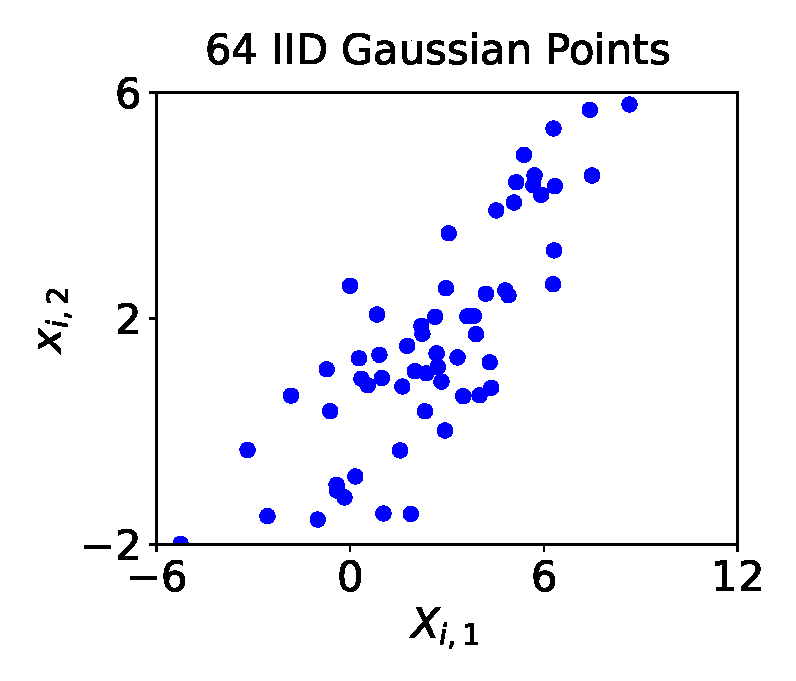
\includegraphics[height = 3.0cm]{ProgramsImages/Gauss_IID.eps}
	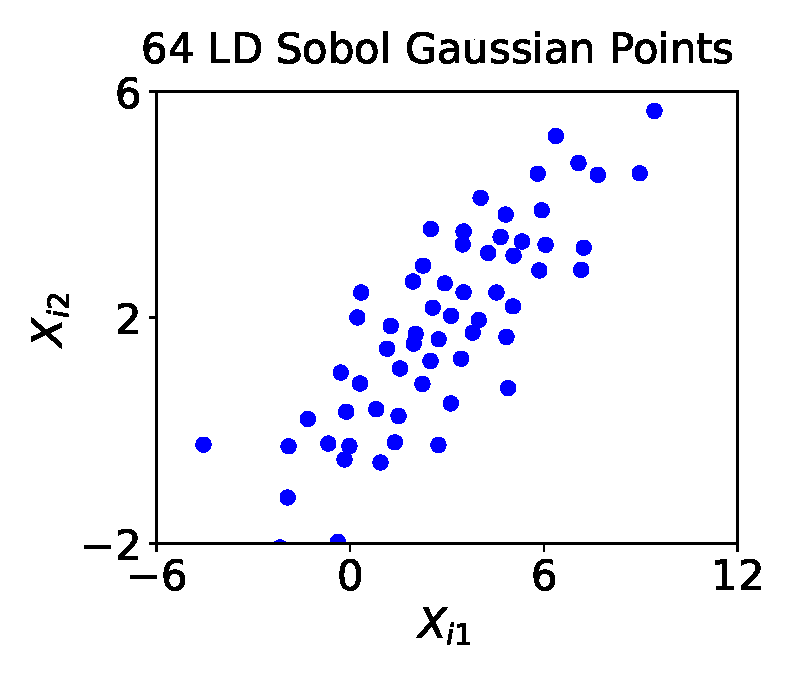
\includegraphics[height = 3.0cm]{ProgramsImages/Gauss_Sobol.eps}
	\caption{IID Gaussian (left) and Sobol'  points transformed to mimic a Gaussian distribution (right).  The LD points better represent the Gaussian distribution than the IID points. \label{fig:ld_Gauss}}
	\vspace{-0.3cm}
\end{wrapfigure}

One may generate additional points while reusing the original ones.   QMCPy LD generators are randomized by default to ensure that no points lie on the boundary of the unit cube and to improve the order of convergence of $\hmu_n$ to $\mu$ \cite{Owe97}. The \pyinline{TrueMeasure} class automates the transformation required to construct good points that mimic distributions other than standard uniform.  The  inverse  distribution is often used.  \cref{fig:ld_Gauss} displays  IID and Sobol' points  transformed to mimic a multivariate  Gaussian distribution.
%with mean $\begin{pmatrix} 3 \\ 2 \end{pmatrix}$ and covariance matrix $\begin{pmatrix} 9 & 5 \\ 5 & 4 \end{pmatrix}$.  
\begin{pythoncode}
gaussian_ld = qmcpy.Gaussian(qmcpy.Lattice(2), mean = [3,2], covariance = [[9,5],[5,4]])  #specify the distribution parameters
points = gaussian_ld.gen_samples(n = 64)  #construct points
\end{pythoncode}

%%%%%%%%%%%%%%%%%%%%%%%%%%%%%%%%%%%%%%%%%%%%%%%%%
\subsubsection*{\textup{\pyinline{Integrand} and \pyinline{StoppingCriterion}}}
%%%%%%%%%%%%%%%%%%%%%%%%%%%%%%%%%%%%%%%%%%%%%%%%%
One must specify the integrand to compute expectations and multivariate integrals as described in \eqref{eq:mean}.   The original form of the problem may not be convenient for computation.  For example, the Keister integral in \eqref{eq:Keister} can be thought of as an integral of $g$ with respect to the Gaussian distribution with zero mean and covariance $\mI/2$:
\begin{multline} \label{eq:KeisterAlt}
\mu = \int_{\reals^d} \underbrace{\pi^{d/2} \cos( \norm[2]{\bt})}_{g(\bt)}  \, \underbrace{\pi^{-d/2}\exp(-\norm[2]{\bt}^2)\, \dif \bt}_{\caln(\bzero, \mI/2)}
= \int_{\reals^d} \underbrace{\cos( \norm[2]{\bt}) \exp(-\norm[2]{\bt}^2)}_{h(\bt)}  \, \underbrace{\dif \bt}_{\text{Lebesgue}} \\
=   \int_{[0,1]^d} f(\bx) \, \dif \bx \qquad \text{for an appropriate transformation } \bt = \bT(\bx).
\end{multline}
Alternatively, $\mu$ can be thought of as an integral of $h$ with respect to Lebesgue measure.  QMCPy can compute the integral either way.

The first way begins by constructing the Gaussian transformed LD \pyinline{TrueMeasure} instance \pyinline{gs} as described in the previous section.  Next, one defines the function $g$ as in \eqref{eq:KeisterAlt} above.   \pyinline{CustomFun}  constructs an $f$ for which the integral, $\mu$, can be written in terms of the uniform distribution, which the LD sequence mimics.   \pyinline{CustomFun} automatically constructs the transformation $\bT$ in \eqref{eq:KeisterAlt}.
\begin{pythoncode}
gs = qmcpy.Gaussian(qmcpy.Sobol(5), covariance = 1/2)    #choose the Gaussian distribution
def g(t):  #your desired integrand, calculations must be vectorized
	d = t.shape[1]
	g_val = np.pi**(d/2) * np.cos(np.sqrt((t**2).sum(1)))
	return g_val  #size n vector
f = qmcpy.CustomFun(gs, custom_fun = g)
sc = qmcpy.CubQMCSobolG(f, abs_tol = 1e-3)   #stopping criterion must match  points
solution, data = sc.integrate()
\end{pythoncode}

The final stage of the computation requires the construction of a \pyinline{StoppingCriterion} instance, \pyinline{sc}.  The one here is due to PI \FH and \hypertarget{LlAJRlink}{Llu\'is Antoni Jim\'enez Rugama} (\LlAJR) \cite{HicJim16a} and is based on Walsh transformations of the sampled integrand data.  Invoking the \pyinline{integrate} method of \pyinline{sc} yields $\hmu_n$ satisfying error criterion \eqref{eq:error_crit} and a data object containing summary results.

Another way to compute the Keister integral \eqref{eq:KeisterAlt} is to think of it as an integral with respect to the Lebesgue measure.  Again \pyinline{CustomFun} selects a default variable transformation or sampling measure.  The answer from QMCPy is the same as the first way, but this second way takes twice the time.  The choice of variable transformation, $\bT$, that defines $f$ from the original integrand is equivalent to importance sampling.  Automatic and adaptive importance sampling requires further research (see Sec. 3.3).

%%%%%%%%%%%%%%%%%%%%%%%%%%%%%%%%%%%%%%%%%%%%%%%%%
\subsection*{QMCPy Options and Support}
%%%%%%%%%%%%%%%%%%%%%%%%%%%%%%%%%%%%%%%%%%%%%%%%%
QMCPy supports digital nets and lattices with generating vectors from several sources.  There are also stopping criteria based on the work of \FH, \SCTC, and their collaborators \cite{HicEtal14a, HicJim16a, JimHic16a,RatHic19a}.  QMCPy is hosted on GitHub \cite{QMCPy2020a}. Bugs can be reported and features requested on the issues page.  Pull requests can be made by those who wish to add features.  All features are documented \cite{QMCPyDocs} using ReadtheDocs.  Doctests ensure that features work as expected. Features are illustrated by Jupyter notebooks.  \FH gave a tutorial on QMC software---with a focus on QMCPy---at MCQMC 2020 \cite{MCQMC2020QMCPyTut}.  A Google Colaboratory Notebook \cite{QMCPyTutColab2020} is available so that those watching  can try out QMCPy themselves in real time.  \FH, \SCTC, \AO, \AS \MM, and \PR wrote  blogs \cite{QMCBlog} to introduce QMC and QMCPy to the broader community.

\subsection{Educating and Mentoring Cross-Disciplinary Computational Researchers}
Computational mathematics and statistics require the use of others' code, hopefully in the form of well-developed software packages.  New scholars need to be trained not only on how to use such packages, but how to contribute to them as well.  QMCPy students supported by this project will learn to write clean, efficient code that fits the package architecture, is documented, and passes doctests.  Some will learn how to combine code from different packages and even different languages.  QMCPy students will learn about repositories and software engineering tools that need to become second nature, just like Beamer became second nature to many a generation ago, and \LaTeX\ two generations ago.

\cmtS{may need to buff up a bit on DEI (I think this was a comment in prior reviews): } As with past projects, in seeking students, we will give preference to underrepresented minorities, women, and students from colleges where research experiences are rare.  As noted in \cref{sec:PreviousFred}, we have had significant success in mentoring students.  Many undergraduates have enrolled in graduate programs.  Five of \FH's fifteen students who earned PhDs are women, three of whom are academics. A  summer 2021 REU student is Black.  Two of \SM's four current PhD students are women.  

The senior personnel on this project include two women (\SCTC and \YD) and one early-career scholar (\SM).  Our senior personnel and collaborators include folks with diverse backgrounds in mathematics, statistics, and computer science.  The students  that we mentor will also learn to think from these different perspectives.

\cmtS{Further emphasis on multi-disciplinary education for the sciences? Some sample writing below}


\subsection*{Training the Next Generation of {\em Science-Based} Data Scientists}

There is a critical need for individuals who have the computational, mathematical, and algorithmic tools to adeptly work in modern scientific teams, geared towards pushing forward the frontier of scientific knowledge and engineering and technical development through improved science-based data science tools.  Traditional data science has been largely driven by \textit{purely} predictive problems that arise in the tech industry, while \textit{science-based} data science is focused on building realistic models of complex phenomena and obtaining interpretable insights from complex computer and real-world experiments. For the latter, one cannot simply rely on \textit{uninterpretable} black box statistical models, but need to develop tools that incorporate scientific knowledge within modeling, provide scientific interpretability and accurate uncertainty quantification.  Students involved in this project will be given a \textit{multidisciplinary} background in science-based data science, and will learn relevant methods in statistics, mathematics, and computer science.  This will serve them well in transitioning to not just academic research teams but also government and industry positions.



\subsection{Expanding the Scope of QMC Application} \label{sec:scopeapplication} \cmtS{will revise, make more focused on specific scientific applications} By making QMC methods easily accessible, QMCPy will \emph{introduce new application areas} to the benefits of LD sampling.  This will lead to \emph{LD sampling being incorporated} into the software packages used by practitioners in those disciplines. This includes, e.g., PyMC3 \citep{salvatier2016probabilistic} and PyStan \citep{stan2017pystan}, which are popular Python packages for Bayesian statistical modeling and machine learning. The accessibility of state-of-the-art QMC methods will spur on novel advancements in many scientific disciplines. We will focus specifically on three areas:
% A recent application of QMC for UQ is to compute the expectation of a functional of solution of a partial differential equation with random coefficients \cite{HerSch20a}. This has broad applications in engineering problems, e.g., fluid flow through a porous medium.
\subsubsection{Uncertainty Quantification (UQ)} UQ is the science of quantifying and managing uncertainty in computational and physical systems \cite{smartuq, Smi14a}. Since data are typically expensive for UQ, a key focus is the design of sampling points for experimentation. QMC can thus yield great computational savings for UQ (see \cite{HerSch20a} for a convincing application in fluid flows). PI \SM is active in multi-disciplinary collaborations on UQ in aerospace engineering \cite{li2017two,li2018uncertainty,chang2019kernel,yeh2018common,mak2018efficient}, nuclear physics \cite{ji2021graphical,everett2021multisystem,everett2021phenomenological,cao2021determining}, astrophysics \citep{mak2018maximum,zheng2021online,makinformation} and neuroscience \cite{wang2020uncertainty,wang2021sequential}, and we will introduce the benefits of LD sampling for UQ in such disciplines.
\subsubsection{Machine Learning (ML)} Machine learning is a rapidly growing area with broad applications in science and engineering. Given the prevalent use of Monte Carlo for scaling up ML algorithms \cite{Bot2010,friedman2002stochastic,quiroz2018speeding}, QMC will undoubtedly have a significant impact in this area (see \cite{Keller2013a} for a visually stunning application of QMC in image rendering, and \cite{chen2019quasi} for an application of QMC for learning PDEs). In addition to LD big data subsampling (\cref{sec:bigdata}), we will \textit{show the advantages of QMC over IID sampling in cutting-edge ML problems}.

% \AGSNote{the article at https://arxiv.org/abs/1911.01612 is another example of QMC for ML where it learns PDEs by training a neural network with LD samples.}
% \SMNote{need? fill in a few sentences.}
% \subsubsection{Probabilistic Numerics}: 
\subsubsection{Bayesian Methodology} Bayesian methods have become popular due to their principled approach for UQ and decision-making. In addition to expensive sampling problems (\cref{sec:bayes}), we will explore two Bayesian areas which can greatly benefit from QMC. The first is \hypertarget{PNlink}{probabilistic numerics} (\PN), which presumes the input solution of a mathematical problem follows a prior random process, thus allowing for probabilistic inference on the solution. PI \FH along with his former PhD student \JR developed a fast Bayesian cubature method \cite{RatHic19a} using lattice LD sampling.  Our collaborator \TS is a \PN expert. \hypertarget{BOlink}{Bayesian optimization} (\BO) applies \PN for minimizing a black-box objective function.  The next samples are chosen as the optimum of an acquisition function, which can take the form of a high-dimensional integral.  \MM illustrates the advantages of LD sampling for computing an acquisition function in \cite[qEI with QMCPy]{QMCBlog}, and PI \SM has also worked in this area \cite{mak2019analysis,chen2019hierarchical}. We will demonstrate the \emph{efficacy of LD sampling} in \BO and other \PN problems.

% \subsection{New QMC Theory}
% The history of QMC is marked by new applications leading to new theoretical and methodological development.  The success of QMC for a $360$-dimensional financial risk application \cite{PasTra95} spurred the theoretical study of QMC's effectiveness for problems with much higher dimensions than was previously thought feasible, which resulted in dozens of articles (see \cite{NovWoz10a,DicEtal14a} and citations therein).  These applications then propelled the development of multilevel \cite{Gil15a} and multivariate decomposition \cite{KuoEtal17a} methods. Looking forward, QMCPy's success in new applications will \emph{raise new methodological and theoretical questions} that we and others will address.

%%%%%%%%%%%%%%%%%%%%%%%%%%%%%%%%%%%%%%%%%%%%%%%%%
\subsection{Promoting Proper QMC Practice and Code} \label{sec:goodpractice}
%%%%%%%%%%%%%%%%%%%%%%%%%%%%%%%%%%%%%%%%%%%%%%%%%
QMCPy---software, documentation, academic articles, and conference presentations---will \emph{showcase the right way} to do LD sampling.  As an example, the adoption of \PyTorch into QMCPy and the tutorial given by \FH at MCQMC 2020 \cite{MCQMC2020QMCPyTut, ChoEtal22a} prompted a vigorous discussion on the \PyTorch issues site \cite{PyTorchFirstPt2020a} that migrated to the \SciPy issues site \cite{scipySobol2020a}.  \AO, \FH, and other QMC researchers convinced the developers to not omit the first Sobol' point, but to randomize by default.  Keeping the first point preserves the net property of the first $2^m$ Sobol' points and randomization can speed up convergence~\cite{owen2020dropping}. In these discussions, it was pointed out that UQLab \cite{UQLab2014}, OpenTurns \cite{OpenTURNS}, and other packages routinely drop the first Sobol' point, a bad but understandable practice.  The arguments we provided to \PyTorch and \SciPy developers addressed their concerns.  We expect this project to produce fruitful discussions between QMC practitioners, which will promote better practice.

Having the eyes of the QMC community on QMCPy will more \emph{quickly uncover and eradicate bugs}.  \FH found  that randomized \PyTorch Sobol' points fell on the boundaries of $[0,1]^d$, when they never should \cite{PyTorchFirstPt2020a} This was due to a lack of double precision, as discovered by \MM.  \LlAJR found that the Sobol' scrambling in \MATLAB was incorrect.  This was rectified in R2017a.  These examples highlight how having a larger community using a software library leads to higher quality code.


\section{Results from Prior NSF Support} \label{sec:prior_work}

\subsection{NSF-DMS-1522687, \emph{Stable, Efficient, Adaptive Algorithms for
		Approximation and Integration},
	\$270,000, August 2015 -- July 2018} \label{sec:PreviousFred}
%%%%%%%%%%%%%%%%%%%%%%%%%%%%%%%%%%%%%%%%%%%%%%%%%%%%%%%%%%%%%%%%%%%%%%%%%%%%%%%%%%%
Fred Hickernell (\FH, PI) and Gregory E. Fasshauer (\GEF, co-PI) led this project, and \SCTC contributed as senior personnel
Gregory E.  Other contributors were \FH's research students {\YD} ( PhD 2015), \LJ (PhD 2016),
\LlAJR (PhD 2016), \hypertarget{DLlink}{Da Li} (\DL, MS 2016), \hypertarget{JLlink}{Jiazhen Liu} (\JL, MS 2018), JR (PhD 2019), \hypertarget{XTlink}{Xin Tong} (\XT, MS 2014, PhD 2020 at the University of Illinois at Chicago), \hypertarget{KZlink}{Kan Zhang} (\KZ, PhD student), \hypertarget{YZlink}{Yizhi Zhang} (\YZ, PhD 2018), and \hypertarget{XZlink}{Xuan Zhou} (\XZ, PhD 2015).  Articles, theses,
software, and preprints supported in
part by this
grant
include
\cite{ala_augmented_2017,
	ChoEtal17a,
	ChoEtal21a,
	Din15a,
	DinHic20a,
	GilEtal16a,
	Hic17a,
	HicJag18b,
	HicJim16a,
	HicEtal18a,
	HicEtal17a,
	HicKriWoz19a,
	RatHic19a,
	GilJim16b,
	JimHic16a,
	JohFasHic18a,
	Li16a,
	Liu17a,
	MarEtal18a,
	mccourt_stable_2017,
	MCCEtal19a,
	mishra_hybrid_2018,
	MisEtal19a,
	rashidinia_stable_2016,
	rashidinia_stable_2018,
	Zha18a,
	Zha17a,
	Zho15a,
	ZhoHic15a}.

%%%%%%%%%%%%%%%%%%%%%%%%%%%%%%%%%%%%%%%%%%%%%%%%%%%%%%%%%%%%%%%%%%%%%%%%%%%%%%%%%%%
\subsubsection{Intellectual Merit from Prior NSF Support}
\label{previousmeritsubsec}
%%%%%%%%%%%%%%%%%%%%%%%%%%%%%%%%%%%%%%%%%%%%%%%%%%%%%%%%%%%%%%%%%%%%%%%%%%%%%%%%%%%

\FH, \SCTC, \YD, \XT, \YZ developed several adaptive algorithms for univariate integration, function approximation, and optimization \cite{ChoEtal17a,HicEtal14b,  Din15a, Ton14a, Zha18a}.  Those constructed by \FH, \SCTC, \YD, and \XT in \cite{ChoEtal17a} are \emph{locally adaptive}---the nonuniform sampling density is influenced by the function data.  For function approximation, the computational cost of $\Order\left(\sqrt{\norm[1/2]{f''}/\varepsilon} \right)$, where $\varepsilon$ is the error tolerance, and is essentially optimal. 
\FH, \LlAJR, \DL, and \JR developed globally adaptive algorithms for approximating $\int_{[0,1]^d} f(\bx) \, \dif \bx$ based on LD sequences \cite{HicJim16a,HicEtal17a,JimHic16a}. 
\FH, \YD, \LlAJR, and collaborators investigated function approximation problems for Banach spaces, $\calf$, defined by series representations \cite{DinHic20a,DinEtal20a}.  Adaptive function approximation algorithms constructed were shown to be essentially optimal.


%%%%%%%%%%%%%%%%%%%%%%%%%%%%%%%%%%%%%%%%%%%%%%%%%%%%%%%%%%%%%%%%%%%%%%%%%%%%%%%%%%%
\subsubsection{Broader Impacts from Prior NSF Support} \label{prevBIsect}
%%%%%%%%%%%%%%%%%%%%%%%%%%%%%%%%%%%%%%%%%%%%%%%%%%%%%%%%%%%%%%%%%%%%%%%%%%%%%%%%%%%
Publications by \GEF, \FH,  \SCTC, students, and collaborators are listed above.  We have spoken at many applied mathematics, statistics,
and computational science conferences and given colloquium/seminar talks to mathematics and
statistics departments.  \FH co-organized the
2016 Spring Research
Conference, \FH gave an invited tutorial
at MCQMC 2016
\cite{Hic17a}, was a program leader for the SAMSI 2017--18 Quasi-Monte Carlo (QMC) Program, and received the 2016 Joseph F.\ Traub Prize for Achievement in Information-Based Complexity.  This research has been implemented in our open-source library
\GAIL \cite{ChoEtal21a}.  \SCTC has been key in this effort.  \GAIL has been used in the graduate Monte Carlo course taught by \FH and \YD. \GEF, \FH, and \SCTC mentored a number of
research students;  female students include \YD, \LJ, \JL, \XT, and Xiaoyang Zhao (MS 2017).



\subsection{NSF CSSI Frameworks 2004571 (Subaward WSU20076). \cmtS{to add} \textit{X-Ion Collisions with a Statistically and Computationally Advanced Program Envelope (X-SCAPE),} \$696,442, July 2020 -- June 2024.} High-energy colliders study the interaction between subatomic particles and environments produced in the collision of protons with protons, with nuclei, or between two nuclei. The study of such interactions requires an elaborate theoretical, statistical and computational framework. The X-SCAPE collaboration is a multi-disciplinary team of physicists, computer scientists, and statisticians, who are engaged in the construction of such an open-source framework. \SM is a Duke co-PI in this ongoing collaboration (which started in the summer of 2020) and is responsible for leading the statistical developments on the project.

\subsubsection{Intellectual Merit from Prior NSF Support}

The X-SCAPE (JETSCAPE) collaboration has developed the first open-source, end-to-end, modular simulation framework for the high energy sector of heavy-ion collisions and a Bayesian statistical framework to rigorously compare event generators with extensive experimental data. The development of the JETSCAPE framework has led to several firsts: the calculation of the suppression of jets, high momentum hadrons from jets, and high momentum heavy hadrons from jets. It is only in the JETSCAPE analysis that the theory prediction is encapsulated by the data-driven approach. The JETSCAPE manual has already appeared online and been submitted to \textit{Comp. Phys. Comm.}, and five papers \cite{cao2017multistage,kumar2019jetscape,everett2021multisystem,everett2021phenomenological,cao2021determining} and several conference papers \cite{soltz2018bayesian,tachibana2018jet,kauder2019jetscape,park2019multi} have also appeared.

\subsubsection{Broader Impacts from Prior NSF Support}
The primary broader impacts of the X-SCAPE collaboration have been in the training of its graduate students and postdocs. Through regular weekly meetings, collaboration gatherings, and joint projects, a multi-disciplinary, multi-institutional environment is fostered between the experimental and theoretical physicists, computer scientists, and statisticians. The collaboration also strives to influence the training of the wider US nuclear physics workforce, through its annual winter school and workshops. Each gathering consists of about 30 students and young postdocs, who are trained in Monte Carlo event generation, heavy-ion collisions, and extensive hands-on tutorials on the JETSCAPE framework.

\subsection{Co-PI Yuhan Ding has no prior NSF support to report}

\section{Strengths of This Team and Collaboration Plan}
\cmtS{May need further thought on DEI, seems to be increasingly important for grants nowadays.} Our team that combines senior personnel with diverse backgrounds, career stages, and institutions.  We will grow QMCPy into what it should become while providing new theories and methodologies to underpin our new algorithms. The leads and team members for each topic are identified above, along with the years for each task.  The senior personnel---together with our students and collaborators---will have regular meetings to share our progress and brainstorm next steps. These will be held both at our own institutions and via video conference among institutions.

\subsection{Senior Personnel}
\FH has been the lead PI on the GAIL \cite{ChoEtal21a} \MATLAB software project that contains many of the stopping criteria incorporated into QMCPy.  His expertise is in the numerical analysis of QMC and other algorithms for multivariate problems as well as theoretically justified adaptive numerical algorithms.  As a former editorial board member for major computational mathematics journals, a Fellow of the Institute of Mathematical Statistics, and a co-leader of SAMSI's program on QMC in 2017-18, \FH understands the interface between computational mathematics and statistics.

\SM is a statistician who became quite familiar with QMC, having served as a Working Group Leader on the aforementioned SAMSI program led by \FH. He is an Assistant Professor of Statistical Science at Duke, specializing in Bayesian computation, big data analytics, and computer experiments. As an Associate Editor for \textit{Technometrics} (a top engineering statistics journal), and the recipient of major awards from the American Statistical Association, \SM provides expertise on statistical theory, methodology and applications. \SM will lead the activities at Duke and oversee the proposed efforts on MLQMC, big data analytics, and Bayesian modeling.

% He also has experience in software library development, having authored four \textsc{R} packages \cite{support,minimaxdesign,cmenet,atmopt} on the Comprehensive R Archive Network (CRAN).

\YD is an associate teaching professor at Illinois Tech, who teaches Monte Carlo methods in finance and programming for data analytic. She is experienced in the theory and implementation of QMC and adaptive algorithms, and is one of the main developers of the GAIL project.

% She is familiar with QMC methods and has started using  QMCPy in her course.

\SCTC is a computational mathematician and engineer, currently serving as the Chief Data Scientist at Kamakura Corporation, a leading financial risk-software company.  She is a research associate professor at Illinois Tech.  \SCTC has co-led the GAIL and QMCPy projects and is an expert in best engineering practices for numerical software.  She is a co-winner of the 2011 Society for Industrial and Applied Mathematics Activity Group on Linear Algebra best paper prize.


\subsection{Students}  \AS began his applied mathematics PhD studies at Illinois Tech in Fall 2021 after completing a dual BS/MS degree at Illinois Tech and doing a large majority of the coding of QMCPy  to date. \IJi and \TT are 3rd year Statistical Science PhD students at Duke University, working on theory and methods for computer experiments, uncertainty quantification, Bayesian modeling and QMC, with applications to heavy-ion and nuclear physics.
PhD students supported by this project will work with the senior personnel to address major algorithmic and theoretical issues.  Undergraduate students will focus on new features or use cases that can be implemented mostly over the course of a summer.  They will be mentored by senior personnel and PhD students. 

\subsection{Collaborators}
\MM convinced his company to fund the early development of QMCPy.  He wanted to spread the advantages of LD sampling to the tech industry. \MM will advise us on the continued development of QMCPy, and continue to help us spread the word among his network in the machine learning community.
\DN has created, coded, and published a number of algorithms for constructing LD generators.  He is expert on efficient code.
\AO has engaged with the PIs in conversations about QMC for many years.  He is particularly an expert in randomized QMC.  \AO has taken a keen interest in QMCPy and will put forward new QMC use cases, advise on software features to be included, and possibly collaborate on joint publications with the PIs. 
\PR has wide experience in multi-level methods and heavy duty applications of QMC.
\TS will provide expertise on two application domains for QMCPy.  The first is \PN, a Bayesian approach to numerical tasks such as cubature.  The second is the use of QMC methods to train metamodels for heterogeneous (i.e. mixed atomistic-continuum) systems, which is of particular interest in Warwick's EPSRC Centre for Doctoral Training in Modelling of Heterogeneous Systems.

%\end{document}

\newpage
\clearpage
%\pagenumbering{arabic}
\setcounter{page}{1}
%\renewcommand{\thepage}{D-\arabic{page}}

\bibliographystyle{spbasic}


{\renewcommand\addcontentsline[3]{}
\renewcommand{\refname}{{\Large\textbf{References Cited}}}                   %%
\renewcommand{\bibliofont}{\normalsize}

\bibliography{FJH23,FJHown23,simon,choi}
\end{document}


\iffalse
https://media.ed.ac.uk/playlist/dedicated/51612401/1_0z0wec2z/1_jkdkrau0

https://drive.google.com/file/d/1UfZinskltBhhAQcYFAzf26FIPFje5aM-/edit

\fi

\iffalse
\subsection{Uncertainty Quantification}
Uncertainty quantification is the science of quantifying, characterizing, tracing, and managing uncertainty in computational and real worlds systems \cite{smartuq, Smi14a}. Since data from such systems are typically expensive to simulate or collect, a key focus in this area is the sampling design for data collection, which can greatly benefit from QMC methods.

A recent application of QMC for uncertainty quantification is to compute the expectation of a functional of solution of a partial differential equation with random coefficients \cite{HerSch20a}. This has broad applications in engineering problems, e.g., fluid flow through a porous medium. \SMNote{emphasize win here} QMCPy will implement a typical use case, which may show how to link QMCPy code with a PDE solver from another package. The PI \SM has done extensive work on uncertainty quantification, for rocket engine design \cite{li2017two,li2018uncertainty,chang2019kernel,yeh2018common,mak2018efficient}, neuroscience modeling \cite{wang2020uncertainty}, and active learning \cite{mak2018maximum}. We will explore the performance of LD sampling for these applications.
\fi


\iffalse
A perspective is that we transform our sampling points to mimic the original distribution, $F$, and work with  the error bound derived by \FH in \cite{Hic99a}:
\begin{equation}
	\abs{ \mu  - \frac 1n \sum_{i=1}^n g(\bT(\bX_i))} \le  D(\{\bT(\bX_i)\}_{i=1}^n,F ) \norm[\calg]{g - \mu},
	\label{eq:kerdisc}
\end{equation}
where the discrepancy $D(\{\bT(\bX_i)\}_{i=1}^n,F )$ is a distance between the empirical distribution of the transformed points and the distribution defining the integral.    This discrepancy is defined in terms of the reproducing kernel, $K$, for the Hilbert space $\calg$.  The advantage of this approach is that it may be easier to determine whether $g- \mu$ has a small $\calg$-norm than determine whether $f_\bT-\mu$ has a small $\calf$-norm.

There is no theory that says when small  $D(\{\bX_i\}_{i=1}^n)$ implies small  $D(\{\bT(\bX_i)\}_{i=1}^n,F )$.  Indeed our recent study \cite{LiKanHic20a} suggests that this is not always the case.  We will derive conditions under which the transformation of low discrepancy points yields low discrepancy points.  This will involve assumptions on the reproducing kernel $K$ and the distribution $F$.

\fi

\iffalse
\begin{wrapfigure}{r}{0.4\textwidth}
	\centering
	\vspace{-1ex}
	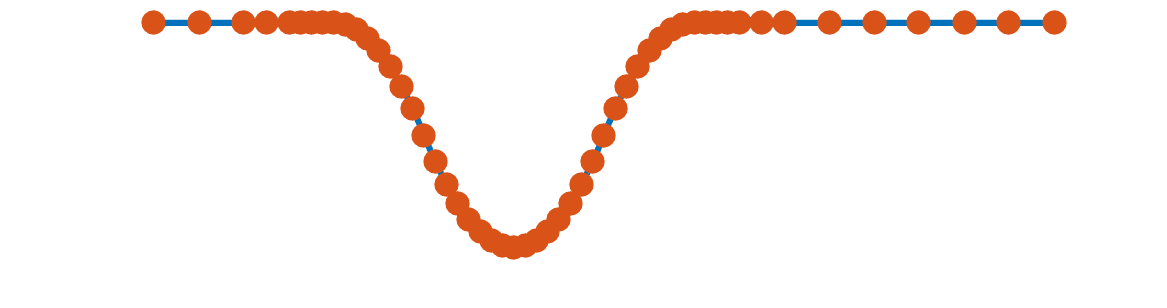
\includegraphics[width = 0.4\textwidth]{ProgramsImages/sampling-funappxg.png}
	\\
	
\includegraphics[width = 0.4\textwidth]{ProgramsImages/sampling-funming.png}
	
	\vspace{-2ex}
	\caption{The function data ({\color{\MATLABOrange}$\bullet$}) for the locally adaptive
		function approximation (top) and minimization (bottom) algorithms in \cite{ChoEtal17a}.  Sampling is denser where $\abs{f''}$ is larger.  For minimization it is also denser where the function values are smaller. \label{localadaptfig}}
\end{wrapfigure}
\fi


%%%%%%%%%%%%%%%%%%%%%%%%%%%%%%%%%%%%%%%%%%%%%%%%%
\subsubsection{Speed-Up} [Years 2--3] \label{sec:speedup}
%%%%%%%%%%%%%%%%%%%%%%%%%%%%%%%%%%%%%%%%%%%%%%%%%
Python's advantages are ease of coding and the rapidly growing code base.  However, Python code does not execute particularly quickly.  Python can be made to execute more quickly by re-writing it in C or utilizing GPUs.  For example, this is done for some of the \PyTorch code.  We will speed up critical QMCPy code by \emph{re-writing it in C}.

There have been attempts at parallel implementations of LD sequences \cite{LiMul00a,OktSri02, SchUhl01,WanEtal06a,LiuHic04a}.  \TensorFlow \cite{tfqf2021a} implements Sobol' sequences using GPUs.  However, parallel or GPU implementations have issues with load balancing. Does one give different processors different segments of the same LD sequence?  Or does one combine the results of several randomized LD sequences, each from a different processor?  We will \emph{implement LD sequences taking advantage of multiple cores} of the same CPU.  We will also explore the possibility of GPU implementations.  Python parallel computing resources \cite{ParallelPython} such as Numba \cite{Numba} will prove invaluable.

%%%%%%%%%%%%%%%%%%%%%%%%%%%%%%%%%%%%%%%%%%%%%%%%%
\subsubsection{Playing Well with Other Python Libraries} [Years 1--2] \label{sec:playwell}
%%%%%%%%%%%%%%%%%%%%%%%%%%%%%%%%%%%%%%%%%%%%%%%%%
When it makes more sense to \emph{write wrappers} around the code in other Python libraries to make them compatible with QMCPy, we will.  E.g., \SciPy \cite{SCIPY} has a wealth of probability distributions, some with inverse distribution functions, which can be used for the variable transformations, $\bT$, required to obtain a QMC-friendly integral over the unit cube from the original integral (see \eqref{eq:KeisterAlt}, for an example of a $\bT$):
\begin{equation} \label{eq:imp}
	\mu = \int_{\reals^d} g(\bt)  \, \lambda(\bt) \dif \bt
	=   \int_{[0,1]^d} f_{\bT}(\bx) \, \dif \bx \qquad \text{for an appropriate transformation } \bt = \bT(\bx).
\end{equation}
By the same token, those methods in QMCPy that become more widely accepted will be pushed into the broad-scope libraries such as PyTorch \cite{paszke2019pytorch}, SciPy \cite{virtanen2020scipy}, TensorFlow \cite{tfqf2021a}.


%%%%%%%%%%%%%%%%%%%%%%%%%%%%%%%%%%%%%%%%%%%%%%%%%
\subsubsection{Richer LD Sequence Generators } [Years 1--2] \label{sec:richLD}
%%%%%%%%%%%%%%%%%%%%%%%%%%%%%%%%%%%%%%%%%%%%%%%%%
Although QMCPy already includes the most popular LD sequences, we will implement more flexibility.  We will expand our generators to include \emph{higher-order digital sequences} \cite{Dic09a, Dic11a}, which yield  faster convergence rates  $n \to \infty$ for smooth integrands, such as those arising in computing multivariate probabilities.  Higher-order nets are not yet available in popular libraries.

For flexibility, the random digital scrambling and shifting of digital nets will be implemented so that either one or both can be turned on or off.  Linear matrix scrambling (LMS) \cite{Mat98,HonHic00a} is the simpler and more common method for randomizing digital sequences (e.g., the Sobol' sequence).  The original nested uniform scrambling (NUS) proposed by \AO \cite{Owe95} requires more complex code and a longer computation time, but it has a \CLT  \cite{Loh01}.  We will \emph{implement NUS} in QMCPy.

Implementing a richer class of LD sequence generators with QMCPy's growing set of use cases will allow us to test which LD sequence generators perform better in practice, e.g., Niederreiter vs.\ Sobol' or LMS vs.\ NUS. If we detect that certain sequences or scrambling methods substantially outperform in practice, then we will develop a \emph{theoretical description} of when that happens.

%%%%%%%%%%%%%%%%%%%%%%%%%%%%%%%%%%%%%%%%%%%%%%%%%
\subsubsection{Stopping Criteria for MLQMC Cubature} \label{sec:stopML}
[Years 1--3]
%%%%%%%%%%%%%%%%%%%%%%%%%%%%%%%%%%%%%%%%%%%%%%%%%
For high or infinite-dimensional integration problems, the computational cost of the integrand is often proportional to $d$, which makes the cost of the sample mean $\Order(dn)$.  Multilevel (Q)MC \cite{Gil15a} decomposes the original integral into a sum of several integrals with different numbers of variables, $d_1 < \dots < d_L$.  The total cost is then $\Order(d_1 n_1 + \cdots + d_L n_L)$. When done well, error criterion \eqref{eq:error_crit} can be met for a decreasing sequence $n_1 > \dots > n_L$, which results in an overall large cost savings compared to a single level (Q)MC algorithm requiring $\Order(d_Ln_1)$ operations. We will \textit{strengthen} QMCPy's rudimentary MLQMC, including extending the theory and implementation of the single level stopping criteria developed by PI \FH, \SCTC, and their collaborators \cite{HicEtal14a,HicJim16a,JimHic16a,HicEtal17a,RatHic19a} to the multilevel case.


